%%%%%%%%%%%%%%%%%%%%%%%%%%%%%%%%%%%%%%%%%%%%%%%%%%%%%%%%%%%%%%%%%%%%%%%%%%
% NOTE: THIS IS A ROUGH TEMPLATE THAT WILL MOST LIKELY NEED CHANGES TO
% CONFORM TO YOUR INDIVIDUAL SITUATION
% THERE IS NO GUARANTEE OF ACCURACY OR COMPLETENESS TO THE TEMPLATE
%%%%%%%%%%%%%%%%%%%%%%%%%%%%%%%%%%%%%%%%%%%%%%%%%%%%%%%%%%%%%%%%%%%%%%%%%%

\documentclass[12pt,a4paper,twoside,openright,final,titlepage]{report}
\usepackage[utf8]{inputenc}
\usepackage{amsmath}
\usepackage{amsfonts}
\usepackage{amssymb}
\usepackage{makeidx}
\usepackage{graphicx}
\usepackage{layout}
\usepackage{lscape}
\usepackage{xfrac}
\usepackage{tabularx}
\usepackage{rotating}
\usepackage{longtable}
\usepackage{makecell}

\usepackage{multirow}
\usepackage{bm} % for bold math symbols (incl. Greek letters) with \bm{}
\usepackage{booktabs}

%\usepackage{todonotes}
\usepackage[colorlinks=true,
							citecolor=black,
							linkcolor=black,
							urlcolor=red,
							linktocpage=true,
							hyperfootnotes=false]{hyperref}

\usepackage[square,numbers,sort&compress]{natbib}
\setlength\bibhang{.3in}

% --------------------- Table in Ch2 ---------------------
\usepackage{booktabs}
\usepackage{multirow}
\usepackage{makecell}
\usepackage{tabularx}
\usepackage{array}
\usepackage{tablefootnote}
\usepackage{xcolor}
\usepackage{pifont}

\newcommand{\cmark}{\textcolor{green!50!black}{\ding{51}}}
\newcommand{\xmark}{\textcolor{red!70!black}{\ding{55}}}
\newcommand{\warn}{\textcolor{orange!90!black}{$\blacktriangle$}}

\newcolumntype{Y}{>{\raggedright\arraybackslash}X}
% --------------------- Table in Ch2 ---------------------

\usepackage{lineno}
\usepackage{setspace}
\onehalfspacing
\usepackage{microtype}
\usepackage{color}
\usepackage{fancyhdr}
\usepackage[labelfont=bf,font=small]{caption}

% For electronic submission use:
\usepackage[inner=3cm,outer=3cm,top=2cm,bottom=2cm]{geometry}
% For printing use:
% \usepackage[inner=4cm,outer=2cm,top=2cm=bottom=2cm]{geometry}


\renewcommand{\chaptermark}[1]{\markboth{\MakeUppercase{\thechapter. #1 }}{}}
\renewcommand{\sectionmark}[1]{}
\fancyhf{}
\fancyhead[RO]{\bfseries\rightmark}
\fancyhead[LE]{\bfseries\leftmark}
\fancyfoot[C]{\thepage}
\setlength{\headheight}{14pt}
\pagestyle{fancy}

\newcommand\frontmatter{\pagenumbering{roman}}
\newcommand\mainmatter{\cleardoublepage\pagenumbering{arabic}}

\newenvironment{chapabstract}{%
	\begin{center}%
		\singlespacing
		\bfseries ABSTRACT
	\end{center}}%
	
\begin{document}
	\hypersetup{pageanchor=false}
	
%	\layout
	\begin{titlepage}
		\centering
		\vfill
		\textit{This thesis is presented for the degree of Doctor of Philosophy of The University of Western Australia}\\
		\vskip 1cm
		{\bfseries\Large
				Recovering Musical Dynamics for Expressive Automatic Music Transcription \\}
		
		\vskip1.5cm
		
		
\includegraphics[width=.40\linewidth]{UWA_new}
		\vskip 2cm	
		Zhanhong HE\\
		B.Sc. in FieldA; B.Sc. in FieldB; M.Sc in FieldC \\
		February 2016\\
		\vskip .5cm
		Department of Electrical, Electronic and Computer Engineering\\
		Electrical Engineering\\
		% 2026\\
%% 		\vskip 1.5cm
% 		\textbf{Supervisors:} 
% 		    Dr. FirstName LastName (Coordinating)\\
% 			Prof. Dr. FirstName LastName\\
% 			Prof. Dr. FirstName LastName\\
% 			Prof. Dr. FirstName LastName\\
	\end{titlepage}
	%\maketitle
	\frontmatter
%	\linenumbers
	\clearpage
	\thispagestyle{empty}
	\phantom{a}
	\vfill
	\vfill
    
	\include{Declaration/declaration}

    
	\begin{abstract}

		Automatic music transcription has achieved significant progress in note transcription. Yet note events alone do not provide enough expressiveness. This thesis establishes musical dynamics as the primary target for expressive AMT, treating note-level MIDI velocity and score-level dynamics as complementary representations. To this end, we propose a unified label-recovery framework evaluated across three practical settings. 
        
        For symbolic velocity completion, we infer missing velocities in flat MIDI files without altering note timing. We achieve this using an attention U-Net inspired by the image colorization, combined with a feature sparsity-aware loss, validating its impact through objective metrics and human listening tests.
		
		We refine audio-based velocity estimation using musical scores as a structural prior. We propose a lightweight score-informed Transformer that achieves leading performance on piano datasets, demonstrating strong robustness to audio-score misalignment.
        
        We predict beat-synchronous score dynamics directly from audio. By utilizing perceptually grounded loudness features and multitask network, this joint estimation approach produces practical dynamics that can be seamlessly integrated into existing scores.

        Finally, we extend our velocity estimation framework beyond the piano. To overcome the scarcity of non-piano MIDI velocity labels, we employ differentiable neural proxies of soundfonts. This enables supervised model training on synthesised audio, successfully bypassing the need for ground-truth MIDI velocity data.
	\end{abstract}
	
	\chapter*{\Large Acknowledgments}
% \enlargethispage{2\baselineskip} \Large

First, I would express my deepest gratitude to my supervisor, Professor Roberto Togneri. His coursework unit is the most clearly one I got during my Bachelor study, and he shows me the light to step-in this journey. With many times of my wasting time consultant, he always kind, and never complained once. Same gratitude to my supervisor Professor Defeng (David) Huang. Since Roberto's retirement, and even thought our topic is not such closed, he read what I wrote in-depth, undoubtly a expertise and professional. In Chinese language, we said the Teachers is like our fathers, and this is my ultimately lucky to have both of them.

Same deepest gratitude goes to my family and relatives. My parents, Weihu He and Weili Chi, what they give me can never pay back. I got many happiness from my sister, Min Hu, and her families: Wen He, Jiahui, Jiaxuan, Jennie, and Jiacheng. Talking with them is the most relaxable time for me. The same warmth goes to my aunt, Xinyun He, who has been like a second mom to me, to her husband, and to my elder brother, Jie Hu, who brought me to university. I share my happiness with my younger brother, Zhanpeng He, who is ongoing graduate and being a professional writer, and my warmest uncle, Weida He, all along his family. I have being overseas too long, and families left along my way. I hope they are well in the heaven.

A special thanks to my partner, Hanyu Meng. She is take over my boring life, and make every day colorful. We have the same topic, similar research interest, and we can always have a deep discussion and make every day joyful and productive. I am so lucky to have her, and I will always be grateful for her support and love.

I would also like to thank my colleagues and friends in UWA, who have been a great support system throughout my PhD journey. Yuliang. Zhihui and Kaibu...

Lastly, my sincere appreciation goes to the Graduate Research School and the EECE administration, Leila Easter, Lea Towler, along with many other warm and supportive members. Their responses were always prompt, helpful, and kind. Staying in UWA has felt like a family to me, and I will always remember and miss my time here. This research was carried out while the author was in receipt of a University of Western Australia International Fee Scholarship (UIFS) and a University Postgraduate Award (UPA). I sincerely thank the University for this financial support, which allowed me to pursue research topics that I found interesting without the financial pressure. I am also grateful to UWA High Performance Computing and IT (HPC-IT) for their strong support. The team consistently provided wholehearted assistance to our research, which was essential in completing my PhD.
	
    \section*{\Large Authorship Declaration: Co-authored Publications}
This thesis contains work that has been published and/or prepared for publication. 
\vskip 0.5cm
	
\begin{tabular}{@{}p{\dimexpr\textwidth-2\tabcolsep\relax}@{}}
\textbf{Details of the work:} \\
\textbf{Zhanhong He (60\%)}, David Cooper (20\%), Defeng (David) Huang (10\%), Roberto Togneri (10\%),\\
``Filling MIDI Velocity using U-Net Image Colorizer,''\\
\emph{Proc.\ 17th Int.\ Symp.\ Computer Music Multidisciplinary Research (CMMR)},\\
pp.~949--960, 2025.\\
% arXiv:2508.07751. DOI: 10.48550/arXiv.2508.07751.\\ %[0.3cm]
\textbf{Location in thesis:} \\
{[insert chapter/section/page range, e.g., Chapter~X, Section~Y, pp.~AA--BB]}\\%[0.3cm]
% \textbf{Student contribution to work:} \\
% {[insert text: describe precisely what you contributed (e.g., problem formulation, model design, implementation, experiments, evaluation, writing, revisions)]}
%\\[0.3cm]
%\textbf{Co-author signatures and dates:} \\
%David Cooper:\ \rule{6cm}{0.4pt}\ \ \ Date:\ \rule{3cm}{0.4pt}\\
%Defeng Huang:\ \rule{6cm}{0.4pt}\ \ \ Date:\ \rule{3cm}{0.4pt}\\
%Roberto Togneri:\ \rule{6cm}{0.4pt}\ \ \ Date:\ \rule{3cm}{0.4pt}
\end{tabular} 
	
\vskip 0.5cm
	
\begin{tabular}{@{}p{\dimexpr\textwidth-2\tabcolsep\relax}@{}}
\textbf{Details of the work:} \\
\textbf{Zhanhong He (60\%)}, Hanyu Meng (20\%), Defeng (David) Huang (10\%), Roberto Togneri (10\%),\\
``Joint Estimation of Piano Dynamics and Metrical Structure with a Multi-task Multi-Scale Network,''\\
\emph{Proc.\ IEEE International Conference on Acoustics, Speech, and Signal Processing (ICASSP)},
p. TBD, 2026.\\
% arXiv:2510.18190. DOI: 10.48550/arXiv.2510.18190.\\%[0.3cm]
\textbf{Location in thesis:} \\
{[insert chapter/section/page range, e.g., Chapter~X, Section~Y, pp.~AA--BB]}\\%[0.3cm]
% \textbf{Student contribution to work:} \\
% {[insert text: describe your contribution vs.\ co-authors (methods, data, experiments, writing, etc.)]}
%\\[0.3cm]
%\textbf{Co-author signatures and dates:} \\
%Hanyu Meng:\ \rule{6cm}{0.4pt}\ \ \ Date:\ \rule{3cm}{0.4pt}\\
%David Huang:\ \rule{6cm}{0.4pt}\ \ \ Date:\ \rule{3cm}{0.4pt}\\
%Roberto Togneri:\ \rule{6cm}{0.4pt}\ \ \ Date:\ \rule{3cm}{0.4pt}
\end{tabular} 
	
\vskip 0.5cm
	
\begin{tabular}{@{}p{\dimexpr\textwidth-2\tabcolsep\relax}@{}}
\textbf{Details of the work:} \\
\textbf{Zhanhong He (80\%)}, Roberto Togneri (10\%), Defeng (David) Huang (10\%),\\
``Score-Informed Transformer for Refining MIDI Velocity in Automatic Piano Transcription,''\\
Under review (\emph{Sound and Music Computing (SMC) Conference}), p. TBD, 2026.\\ arXiv:2508.07757. \\%[0.3cm]
\textbf{Location in thesis:} \\
{[insert chapter/section/page range, e.g., Chapter~X, Section~Y, pp.~AA--BB]}\\%[0.3cm]
% \textbf{Student contribution to work:} \\
% {[insert text: describe your contribution vs.\ co-authors]}
%\\[0.3cm]
%\textbf{Co-author signatures and dates:} \\
%Roberto Togneri:\ \rule{6cm}{0.4pt}\ \ \ Date:\ \rule{3cm}{0.4pt}\\
%Defeng (David) Huang:\ \rule{6cm}{0.4pt}\ \ \ Date:\ \rule{3cm}{0.4pt}
\end{tabular} 
	
\vskip 0.5cm
	
\begin{tabular}{@{}p{\dimexpr\textwidth-2\tabcolsep\relax}@{}}
\textbf{Details of the work:} \\
\textbf{Zhanhong He (70\%)}, Hanyu Meng (10\%), Defeng (David) Huang (5\%), Roberto Togneri (5\%),\\
``Beyond Piano: Cross-Instruments MIDI Velocity Estimation with Neural Proxies of SoundFont,''\\
Under review (\emph{ISMIR} Conference), 2026.\\
% arXiv:2510.18190. DOI: 10.48550/arXiv.2510.18190.\\%[0.3cm]
\textbf{Location in thesis:} \\
{[insert chapter/section/page range, e.g., Chapter~X, Section~Y, pp.~AA--BB]}\\%[0.3cm]
% \textbf{Student contribution to work:} \\
% {[insert text: describe your contribution vs.\ co-authors (methods, data, experiments, writing, etc.)]}
%\\[0.3cm]
%\textbf{Co-author signatures and dates:} \\
%Hanyu Meng:\ \rule{6cm}{0.4pt}\ \ \ Date:\ \rule{3cm}{0.4pt}\\
%David Huang:\ \rule{6cm}{0.4pt}\ \ \ Date:\ \rule{3cm}{0.4pt}\\
%Roberto Togneri:\ \rule{6cm}{0.4pt}\ \ \ Date:\ \rule{3cm}{0.4pt}
\end{tabular} 
	
\vskip 0.5cm
	
\begin{tabular}{@{}p{\dimexpr\textwidth-2\tabcolsep\relax}@{}}
Student signature: [insert signature] \\
Date: [insert date]\\
\end{tabular}
	
\vskip 0.5cm
	
\begin{tabular}{@{}p{\dimexpr\textwidth-2\tabcolsep\relax}@{}}
I, [name of coordinating supervisor] certify that the student statements \\
regarding their contribution to each of the works listed above are correct. \\
Coordinating supervisor signature: [insert signature]\\
Date: [insert date]
\end{tabular}

    
	\setcounter{tocdepth}{2}
	\tableofcontents
	\listoffigures
	\listoftables
	\mainmatter
	\hypersetup{pageanchor=true}
	\raggedbottom
	\chapter{Introduction}
\label{ch:introduction}

\newcommand{\IncludeGraphicsOrPlaceholder}[2][]{%
  \IfFileExists{#2}{%
    \includegraphics[#1]{#2}%
  }{%
    \fbox{%
      \parbox[c][0.22\textheight][c]{0.9\linewidth}{%
        \centering Missing figure file\\\texttt{\detokenize{#2}}%
      }%
    }%
  }%
}

A structurally correct sequence of notes is only the foundation of a musical performance. When performers receive a composed score, they do not merely execute a rigid sequence of instructions. They interpret the piece and bring it to expressiveness. A central dimension of this interpretation is musical dynamics. This involves the deliberate shaping of loudness over individual notes, phrases, and larger formal units. Dynamics conveys emotional nuance. It balances voices inside a texture and shapes the direction of a phrase. It is often the clearest signal that separates a convincing human performance from a flat mechanical rendering.

Msical performance is commonly represented in two complementary symbolic forms. The first is MIDI, where note events are paired with note-level control parameters such as velocity. MIDI velocity records the action intensity at note onset. It is precise, machine-readable, and directly editable, mostly comes from the sensor physical measures. The second is the music score, where dynamics is represented by human-readable markings such as \textit{pp}, \textit{p}, \textit{mf}, \textit{f}, \textit{ff}. These markings are relative, context-dependent, and less precise as physical measurements, but they communicate musical intent on a musically meaningful metrical grid. 

Automatic Music Transcription (AMT) aims to bridge human performance audio and symbolic music representations, including MIDI and scores. Driven by deep learning and large aligned datasets \cite{hawthorne2019maestro}, recent AMT systems can transcribe note events with high accuracy. Yet this progress remains asymmetric \cite{amt2019ov}. The field is proficient at recovering what notes are played and when they occur. It is much less mature at recovering how loud those notes are played in terms of the dynamics shaping and other expressive dimensions, as depicted in Figure~\ref{fig:intro_expressive_amt}

This thesis posits that dynamics is a foundational component of expressive AMT. While music expression is multifaceted, dynamics represents the most perceptually salient and practically essential dimension. Unlike a standard transcription that yields flat intensities, a dynamics-aware approach enables expressive rendering and high-quality symbolic corpora curation. By focusing on the robust recovery of score dynamics and MIDI velocity, this work provides a critical layer of musical information.

\begin{figure}[h!]
  \centering
  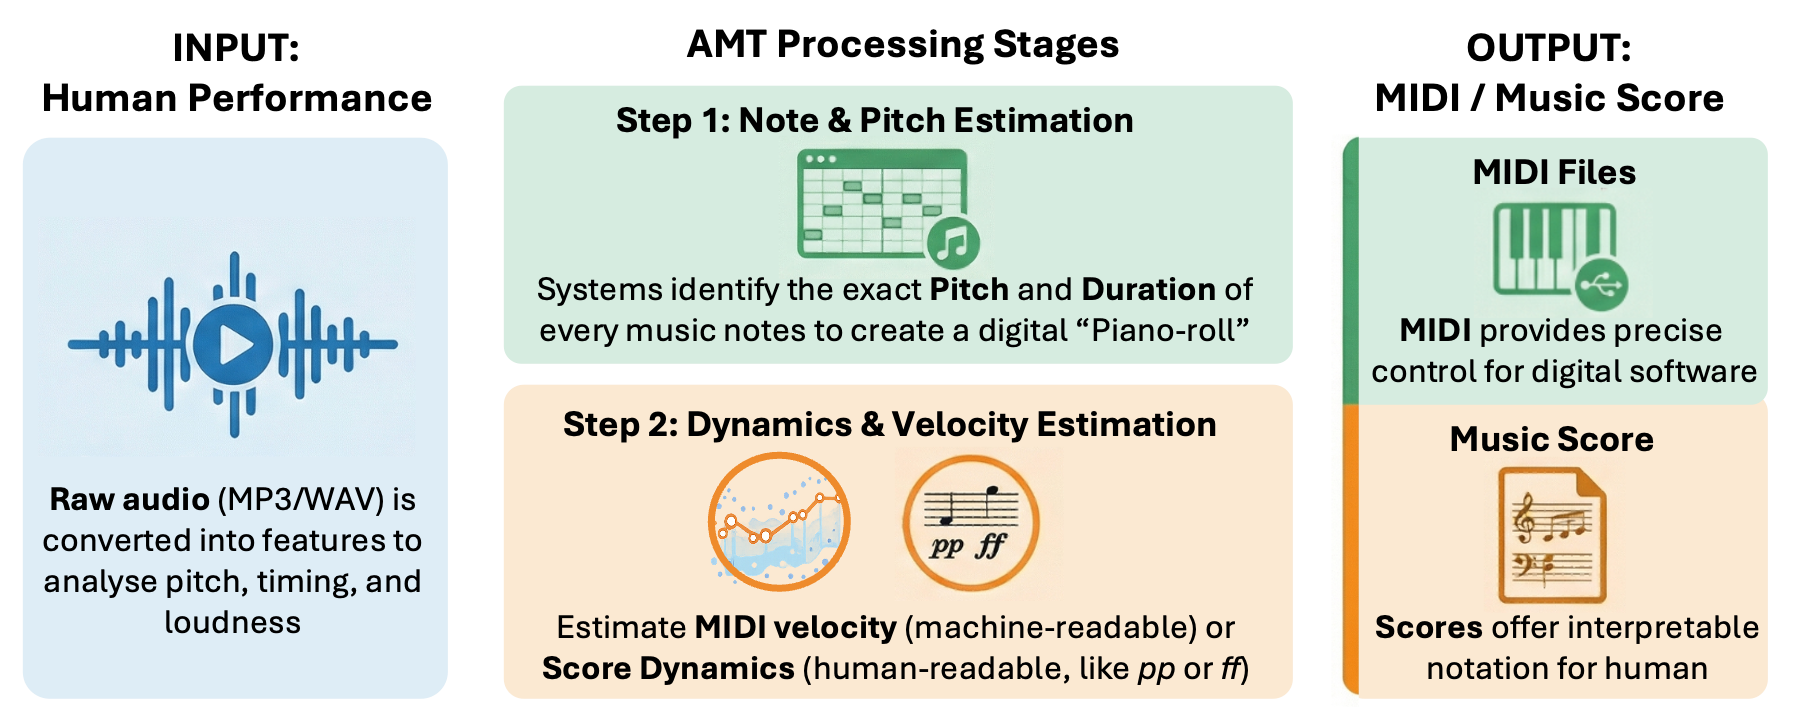
\includegraphics[width=\linewidth]{Chapter_1/figures/AMT.png}
  \caption{The general architecture of an AMT system, illustrating the transformation of raw acoustic audio into foundational note events and expressive dynamic information. The pipeline results are MIDI data and musical scores.}
  \label{fig:intro_expressive_amt}
\end{figure}

\section{Motivation}
\label{sec:motivation}

Transcribing correct pitches and timing is only the foundational step of AMT. Incorporating dynamics into transcription results significantly enhances their capacity to carry expressive intent, taking the form of MIDI velocity or score dynamics. This is not only a technical improvement. Transitioning toward such expressive AMT unlocks significant practical benefits, as outlined below:

\paragraph{MIDI production and expressive rendering.} 
MIDI is the dominant representation in digital music production, supporting efficient editing and flexible rendering. Yet, much software-generated MIDI is created via step input and quantisation, leaving expressive parameters at a lifeless, default constant. Among these, MIDI velocity is one of the most accessible control variables for shaping note intensity and expressive contour \cite{dan2006psy,palamara2020dynamic}. Creators often want to preserve their composed notes and timing. To inject human-like expression, they simply need to adjust velocity values. Still, manual editing is time-consuming and delicate. Developing automated methods for velocity completion becomes an essential step for realistic rendering.

\paragraph{Music education and performance feedback.} 
Score dynamics is also a core pedagogical dimension. In automatic piano performance assessment, dynamics is routinely treated alongside pitch, timing, and rhythm as one of the salient components of performance quality and feedback \cite{kim2022piano}. More recent work on query-based music coaching likewise emphasises that useful educational feedback needs interpretable information about expressive shaping, not only note correctness \cite{zhang2025llaqo,park2025dynvisual}. In many educational scenarios, a reference score is already available together with a student performance audio. This makes score-informed dynamics estimation especially attractive, because the symbolic prior can stabilise the prediction while keeping the feedback musically meaningful.

\paragraph{Expressive data curation by enhancing existing archives.}
A third motivation comes from data curation. Many large-scale music archives provide aligned audio and symbolic content (MIDI sequences or digital scores). However, expressive labels are consistently missing. Velocities are often flattened to a default value, and score dynamic markings are absent or unreliable, limiting the utility of these corpora for downstream applications. Furthermore, a deep semantic gap exists between physical machine measurements (MIDI velocity) and subjective human cognition (score dynamics). Bridging this gap and recovering these missing dimensions is imperative to upgrade static archives into richly expressive datasets.

By contrast, recollecting new datasets from scratch is a costly process constrained by audio-to-score synchronisation challenges, required musical expertise, and copyright restrictions \cite{li2019urmp,foscarin2020asap,morsi2022bottlenecks}. Therefore, this thesis treats \emph{label recovery} as a scalable, principled strategy. By retroactively estimating missing dynamics on existing corpora, we entirely bypass acquisition bottlenecks and annotation ambiguities, unlocking a vast, previously untapped resource for data-driven music research.

\section{Dynamics as a Target in Expressive AMT}
\label{sec:intro:why_dynamics}

Expressive AMT extends beyond recovering mere pitch and onset/offset boundaries to capture the full aspects of a human performance. A comprehensive expressive transcription can be conceptually divided into three primary layers:
\begin{itemize}
\item \textbf{Timing Layer:} Captures the temporal elasticity of a performance, encompassing macro-level tempo variations, beat tracking, inter-onset intervals (IOI), and micro-level articulation.
\item \textbf{Dynamic Layer:} Represents the intensity and energy of the musical execution, bridging physical machine measurements (e.g., MIDI velocity) with semantic cognitive notations (e.g., score dynamic markings).
\item \textbf{Control Layer:} Includes instrument-specific techniques and acoustic modifiers, such as sustain pedaling, vibrato, reverberation, and amplifier configurations.
\end{itemize}
While all three layers are essential for a complete computational understanding of performance, this thesis isolates the \textbf{Dynamic Layer} as its primary expressive target. This focus does not imply that timing or control parameters are secondary. Rather, dynamics is chosen to move AMT beyond note content for three reasons:

\paragraph{Perceptual salience.}
Dynamics is one of the most immediately audible dimensions of expressive performance. Listeners often perceive phrase direction, accent, and balance through intensity change before they perceive subtler aspects such as pedaling or micro-timing. A transcription that omits dynamics therefore omits a central part of musical meaning.

\paragraph{Symbolic editability.}
Compared to complex continuous controls like overdrive (electric guitar) or pedaling (piano), dynamics offers an exceptionally tractable and editable symbolic representation. MIDI velocity serves as a universal, loudness control parameter for all instrumentsin digital audio workstations (DAWs), while score dynamics provide a standard notational device for composition, pedagogy, and performance analysis. This dual nature makes dynamics a robust bridge between low-level MIR outputs and high-level musical practice.

\paragraph{Recoverability across realistic data conditions.}
Many expressive targets require fine-grained, instrument-specific mechanisms, particularly within the Control Layer. They are entirely absent or poorly labeled in existing large-scale music datasets. Dynamics, while challenging to estimate accurately, remains highly recoverable across various practical paradigms. It therefore provides a scalable entry point for advancing expressive AMT without being bottlenecked by instrument-specific data scarcity.

\section{Two Complementary Forms of Dynamics}
\label{sec:intro:two_forms}
Having established dynamics as our primary expressive target, we clarify its two complementary symbolic forms within this thesis, as summerized in Table \ref{tab:intro_two_forms}.

\begin{table}[b]
\centering
\caption{Two complementary forms of dynamics that recur throughout this thesis.}
\label{tab:intro_two_forms}
\fontsize{11pt}{13pt}\selectfont
\setlength{\tabcolsep}{4pt}
\renewcommand{\arraystretch}{1.2}
\begin{tabularx}{\textwidth}{llll}
\toprule
\textbf{Representation} & \textbf{Nature} & \textbf{Temporal Anchor} & \textbf{Primary Carrier} \\
\midrule
MIDI velocity & \makecell[l]{Physical\\measurement} & \makecell[l]{Note-level: isolated value\\at each note} & \makecell[l]{DAWs, electronic\\instruments (synthesisers)} \\
Score dynamics & \makecell[l]{Subjective\\intention} & \makecell[l]{Metrical-level: shared value\\in a beat/phrase} & \makecell[l]{Digital sheet music,\\human performers} \\
\bottomrule
\end{tabularx}
\end{table}

\paragraph{MIDI velocity.}
Originating from the physical sensors of electronic keyboards and pianos, MIDI velocity is a machine-centric measurement of physical intensity. To say it operates as a "note-level" parameter means that every music note from a discrete key strike is assigned an independent, static integer representing its initial strike force. This strict per-note measurement dictates that velocity functions as a discrete loudness control parameter. It is highly granular and absolute within its own scale, yet the resulting loudness highly depends on the acoustic environment and the specific instrument being played. Because MIDI velocity is necessary for MIDI-to-audio playback in DAWs and synthesizers, a common default is set to 64 when it is missing.

\paragraph{Score dynamics.}
Score dynamics represents the subjective cognitive intention of the composer or performer. Instead of attaching to isolated notes, markings like \textit{p} or \textit{crescendo} are conceptually anchored to the underlying metrical structure, acting as shared values across a specific beat or an entire phrase. This segment-level instruction provides a holistic perception of intensity while leaving room for free human interpretation. Because it is structurally aware and musically meaningful, score dynamics is the ideal target for pedagogical feedback and score analysis. In symbolic environments, the default assumption is often that missing score dynamics should be filled with \textit{mf} (mezzo-forte), which is the neutral middle ground of human perceptual loudness. 

\section{Research Gap and Thesis Stance}
\label{sec:intro:gap_stance}

This section point to a narrower and more practical research gap than the general claim that AMT still lacks expressiveness. A recurring paradox in music research is that while structural data (pitch and timing) is increasingly abundant, expressive data remains systematically impoverished. A MIDI file may contain correct note sequences while leaving all velocities ar a default constant. A performance corpus may preserve audio and aligned scores but only sparse, unreliable, or absent dynamic markings. The common is therefore how to recover a missing expressive label layer from data that are already partly specified.

\paragraph{The ontological gap: dynamics must be inferred across representations.}
This is not a simple label-conversion problem. Audio loudness an acoustic and perceptual phenomenon. MIDI velocity is a machine-centric, physical parameter. Score dynamics is a cognitive, context-dependent notation of musical intention. These three forms are related but encodes different concepts. A method that translates one to another must bridge the fundamental gap between objective physical measurement and subjective human cognition.

\paragraph{The ambiguity of ground truth: dynamics is more fragile than notes.}
For note transcription, pitch and onset often remain learnable under moderate changes in instrument, room, or recording conditions. Dynamics ground truth is less stable. Small changes in instruments (timbre), microphone placement, editorial convention, or synthesis setup can alter the apparent relation between sound, MIDI velocity, and score dynamics notation. For non-piano settings, the difficulty becomes sharper because the bottleneck is not ordinary domain shift but missing measurement itself: reliable MIDI velocity labels are rarely available, and in some cases even the ground truth is instrument-dependent.

\paragraph{Fragmented supervision regimes.}
The MIR community lacks a singular, omnipotent dataset that pairs audio with both cognitive score annotations and physical velocity labels. Supervision is deeply fragmented: some corpora provide aligned scores without performance control, while others provide precise velocity data but no human-readable score. A robust thesis on expressive dynamics cannot rely on an idealized, fully supervised data regime. It must systematically address these disjointed data environments.

\paragraph{Thesis stance: label recovery under structural preservation.}
For these reasons, this thesis adopts a unified \emph{label-recovery} perspective. It does not treat the problem as music generation, full expressive rendering, or style transfer. Instead, it asks a narrower, more pragmatic question: when pitch, onset, and often alignment are already trusted, how can the missing dynamics labels be recovered without rewriting the note content or trusted timing? The ultimate goal is to recover labels that remain musically interpretable and directly usable—whether as note-level MIDI velocity for production workflows, or as beat-synchronous score dynamics for pedagogy and analysis.

\section{Unified Thesis Question and Three Core Scenarios}
\label{sec:intro:question}

The thesis is driven by the following question:

\begin{quote}
\textbf{How can musically interpretable dynamics labels be recovered from incomplete, weakly expressive, or weakly supervised music data without rewriting note content or note timing?}
\end{quote}

That question is studied under three core scenarios.

\begin{table}[t]
\centering
\caption{The three core supervision scenarios studied in this thesis.}
\label{tab:intro_scenarios}
\small
\setlength{\tabcolsep}{4pt}
\renewcommand{\arraystretch}{1.15}
\begin{tabularx}{\textwidth}{l X X X X}
\toprule
\textbf{Scenario} & \textbf{Available data} & \textbf{Missing label} & \textbf{Target output} & \textbf{Position} \\
\midrule
S1 & MIDI note sequence & note-level expressive intensity & MIDI velocity completion & Chapter~3 \\
S2 & performance audio + aligned MIDI (score) & reliable note-level expressive intensity & score-informed MIDI velocity refinement & Chapter~4 \\
S3 & performance audio only & human-readable score-facing dynamics and metrical coordinates & beat-synchronous dynamic levels, change points, beats, downbeats & Chapter~5 \\
\bottomrule
\end{tabularx}
\end{table}

\begin{enumerate}
    \item \textbf{Scenario S1: symbolic-only MIDI velocity completion.} The note content and timing are already available in MIDI form, but the velocity is missing or flattened. The goal is to complete note-level velocity from symbolic structure alone.

    \item \textbf{Scenario S2: audio-plus-score velocity refinement.} A performance recording is available together with an aligned score. While the AMT audio-only velocity estimation serves as a plausible but optimizable baseline, the goal is to refine this velocity by using the score as a structural prior.

    \item \textbf{Scenario S3: audio-only score-dynamics recovery.} Only the performance audio is available, and the goal is not raw note-level velocity but beat-synchronous score dynamics. The system must therefore recover dynamic levels together with the metrical structure needed to place them on a symbolic score.
\end{enumerate}

These three scenarios are intentionally ordered from the most controlled setting to the most open one. Scenario S1 isolates dynamics recovery by assuming symbolic notes are already available. Scenario S2 adds real audio context while keeping structural support from a score. Scenario S3 removes that support, moving to a more ambiguous, human-readable target. While these three form the core empirical arc, the thesis will also present a brief exploratory extension (Chapter 6) to investigate whether this velocity learning framework can generalize beyond the piano.

\section{Aim, Scope, and Assumptions}
\label{sec:intro:scope}

The aim of this thesis is to develop stand-alone but conceptually linked methods for recovering dynamics-related labels from real music data. The recovered labels include note-level MIDI velocity, beat-synchronous dynamic levels, change points, beats, and downbeats. The intended outcome is not only stronger AMT-style prediction, but also more expressive and more editable symbolic music for downstream use.

The main scope and assumptions are as follows.

\begin{itemize}
    \item \textbf{Primary empirical focus.} The main experimental focus is piano. This is because reliable note-level velocity ground truth remains concentrated on instrumented pianos particularly by the Yamaha Disklavier systems \cite{hawthorne2019maestro}.

    \item \textbf{Preservation of note content and timing.} The thesis does not aim to rewrite the note sequence. Dynamics is treated as a refinement or annotation layer on top of fixed note events.

    \item \textbf{Two complementary outputs.} The thesis studies both note-level MIDI velocity and beat-synchronous score dynamics. It does not force all expressive information into a single representation.

    \item \textbf{Out-of-scope factors.} The thesis does not attempt full modelling of articulation, pedal, timbre, or micro-timing, except when these factors provide indirect context for dynamics recovery.

    \item \textbf{Beyond piano.} Extending velocity estimation beyond piano is recognised as an important direction because piano-centric datasets create a real bias in expressive AMT. However, large-scale non-piano score-dynamics transcription with human labels remains outside the present thesis scope.
\end{itemize}

\section{Main Contributions}
\label{sec:intro:contrib}

The main contributions of this thesis are as follows.

\begin{itemize}
    \item \textbf{A thesis-level formulation of dynamics-oriented label recovery.} The dissertation argues that dynamics should be treated as a first-class target in expressive AMT and organises the problem around heterogeneous supervision regimes rather than one ideal dataset.

    \item \textbf{A symbolic-only method for note-level velocity completion.} Chapter~3 reformulates MIDI velocity completion as an image-colorisation problem on sparse piano-roll representations. It introduces a U-Net with window attention and a sparsity-aware loss, and shows gains in both objective metrics and listening tests \cite{he2025filling}.

    \item \textbf{A modular score-informed correction strategy for AMT velocity estimation.} Chapter~4 introduces a lightweight Transformer correction module that refines AMT-estimated velocity using an aligned score. The design goal is portability across existing AMT backbones rather than a fully bespoke score-informed system.

    \item \textbf{An audio-only framework for beat-synchronous score-dynamics recovery.} Chapter~5 proposes a compact multi-task multi-scale network that jointly estimates dynamic levels, change points, beats, and downbeats. It combines a perceptually motivated Bark-scale specific loudness front-end with task-aware decoding through MMoE \cite{he2026dynest,ma2018mmoe}.

    \item \textbf{An exploratory beyond-piano study based on proxy supervision.} Chapter~6 investigates cross-instrument MIDI velocity estimation when true labels are scarce. It employs a differentiable proxy for black-box synthesizers as part of the supervision signal. This contribution tests a route beyond the piano domain.
\end{itemize}


\begin{figure}[h]
  \centering
  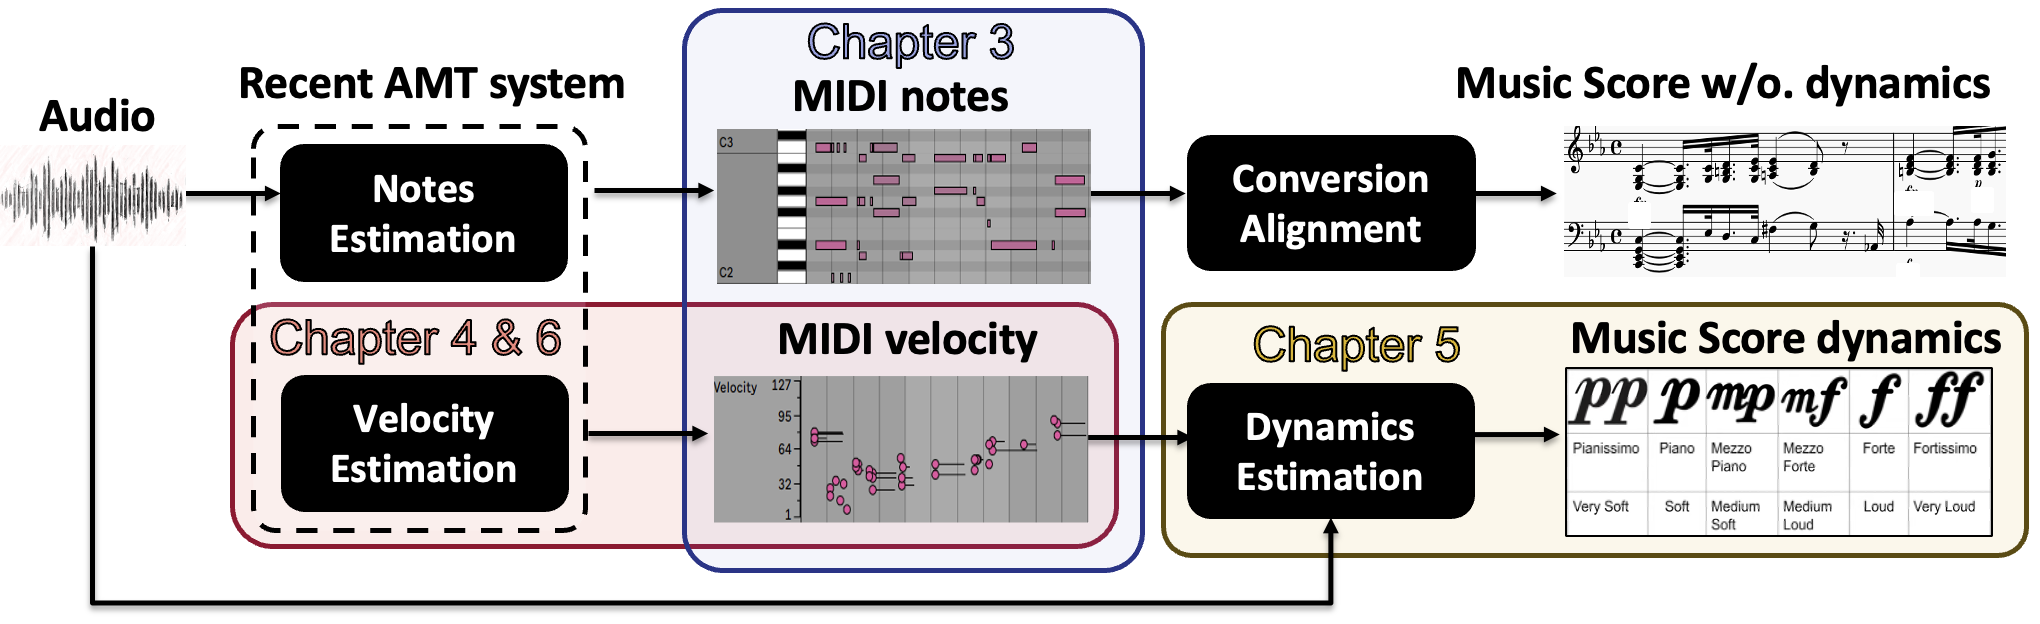
\includegraphics[width=\linewidth]{Chapter_1/figures/Overview.jpg}
  \caption{Shared problem space of the thesis. The dissertation studies dynamics across three linked but non-identical representations: acoustic evidence in audio, note-level performance control in MIDI velocity, and score-facing symbolic intention in notated dynamics.}
  \label{fig:intro_overview}
\end{figure}


\section{Thesis Organisation}
\label{sec:intro:organisation}

Referring Figure~\ref{fig:intro_overview}, the core methodological chapters (Chapters 3--5) preserve the technical contributions of their respective peer-reviewed publications, while expanding the motivation, task-specific related work, and overarching discussion to form a unified narrative. The remainder of the thesis is organised as follows:

\textbf{Chapter~2} establishes the shared conceptual system of the dissertation. It defines what dynamics means across audio, MIDI, and score, and reviewing the AMT models, datasets and evaluation strategies.

\textbf{Chapter~3} addresses Scenario~S1. It formulates symbolic-only MIDI velocity completion as an image-colorisation problem on sparse piano-rolls. Supported by listening tests, it demonstrates that restoring note-level dynamics alone is enough to transform a mechanical MIDI sequence into an expressive, human-like performance, all while keeping the original note content and timing strictly fixed.

\textbf{Chapter~4} addresses Scenario~S2. It introduces a lightweight, portable Transformer correction module that refines AMT-estimated velocity from performance audio using an aligned score as a structural prior. It shows that this approach has better generalisation under dataset shift than AMT baseline, and robustness to audio-to-score misalignment.

\textbf{Chapter~5} addresses Scenario~S3. It proposes an audio-only framework using a multi-task multi-scale network to jointly estimate score dynamic markings and metrical structure, which is the temporal anchor needed to place them into music score.

\textbf{Chapter~6} extends the note-level velocity thread beyond piano. It studies cross-instrument MIDI velocity estimation with proxy supervision. It confronts the dataset bias exposed by earlier chapters by investigating cross-instrument MIDI velocity estimation with proxy supervision, probing the frontier where direct velocity labels disappear.

\textbf{Chapter~7} revisits the unified thesis question, concludes the findings across the four studies, states the limitations clearly, and outlines future directions for expressive AMT.
	% Requires packages: graphicx, booktabs, tabularx
\chapter{Background and Related Work}
\label{ch:background}

This chapter provides the shared foundations for the dissertation. It is not a warehouse of citations. Its task is to define the objects, coordinates, and validity conditions that recur across the later chapters. The chapter therefore focuses on what must be stable across the thesis even though the method chapters are not stages of one end-to-end pipeline.

Section~\ref{sec:bg:dynamics} operationalises musical dynamics across physical sound level, perceived loudness, MIDI velocity, and score-level symbols. Section~\ref{sec:bg:foundations} summarises the deep-learning and MIR ideas that recur across the thesis. Section~\ref{sec:bg:repr} describes the audio, MIDI, and score representations together with the required alignment assumptions. Sections~\ref{sec:bg:threadA} and \ref{sec:bg:threadB} review the two main literature threads of the dissertation: note-level MIDI velocity recovery and beat-synchronous score-dynamics recovery. Section~\ref{sec:bg:common_arch} highlights the reusable method families that recur across chapters. Section~\ref{sec:bg:dataeval} summarises datasets, evaluation, and reproducibility constraints. The chapter ends by converting the literature gaps into explicit thesis requirements.

\section{Musical Dynamics}
\label{sec:bg:dynamics}

The word \emph{dynamics} is used in several related but non-identical ways across music theory, performance research, and MIR. That distinction is not a terminological luxury. It determines what target is being estimated, what evidence is relevant, and what evaluation is legitimate.

\begin{figure}[t]
  \centering
  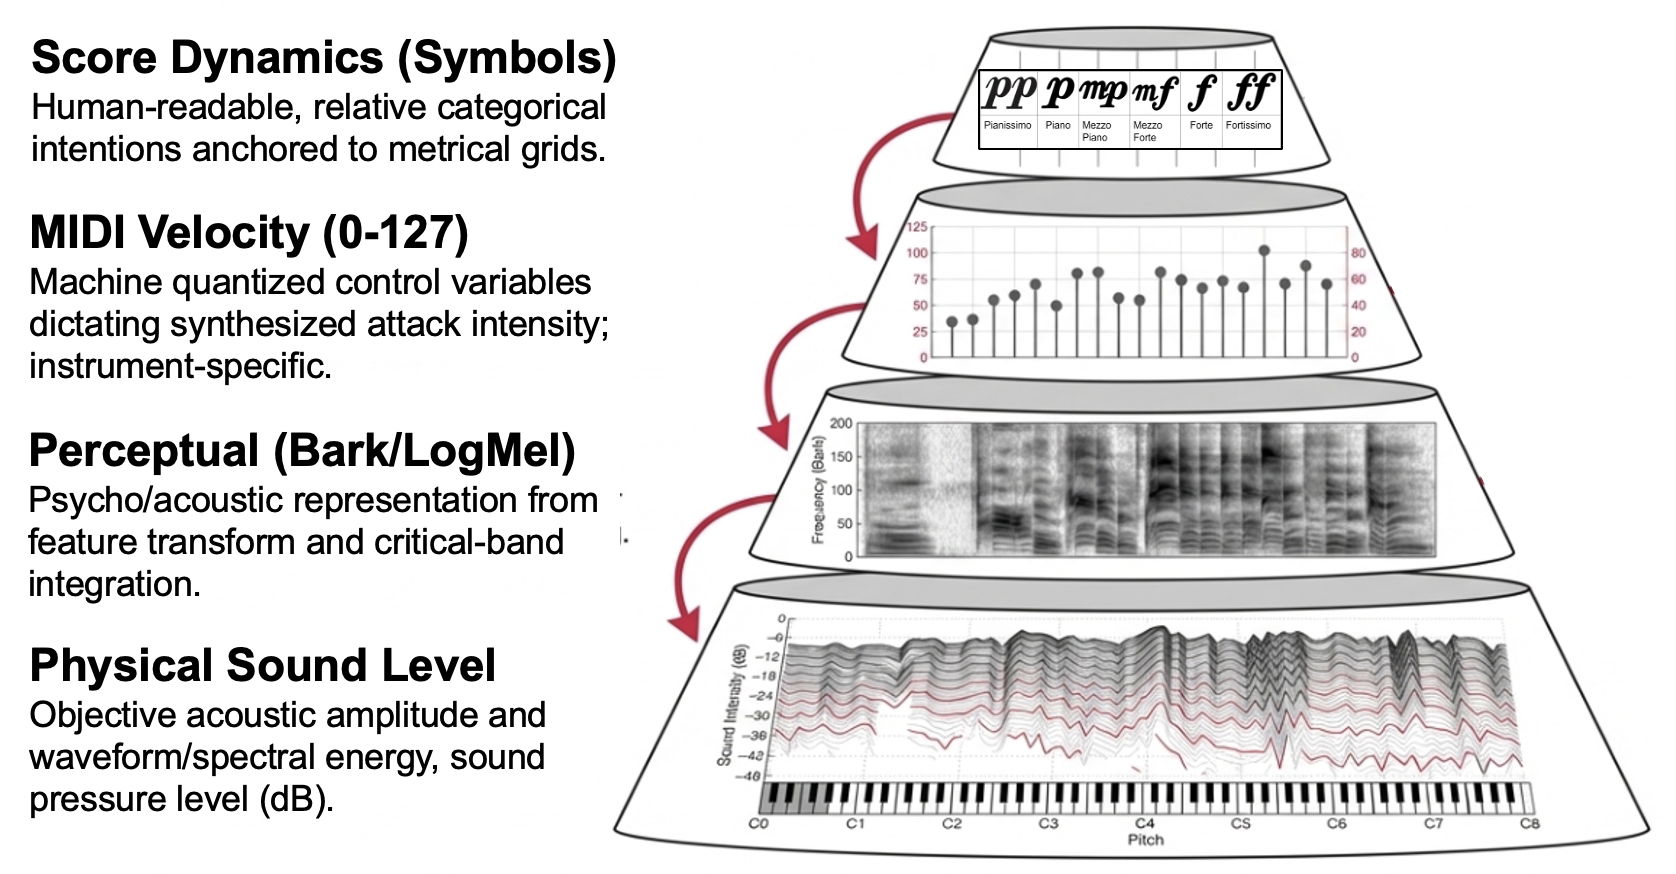
\includegraphics[width=0.9\linewidth]{Chapter_2/figures/dynamics_layers_v1.jpg}
  \caption{Layered view of dynamics used in this thesis. Physical sound level, perceived loudness, MIDI velocity, and score dynamics are linked but not interchangeable. Each transition is many-to-many or instrument-specific.}
  \label{fig:bg_dynamics_layers}
\end{figure}

\begin{table}[t]
\centering
\caption{Three dynamics representations that recur throughout this thesis.}
\label{tab:bg_dynamics_compare}
\small
\setlength{\tabcolsep}{4pt}
\renewcommand{\arraystretch}{1.15}
\begin{tabularx}{\textwidth}{l l X X}
\toprule
\textbf{Representation} & \textbf{Temporal anchor} & \textbf{Main strength} & \textbf{Main limitation} \\
\midrule
Audio loudness & frame-wise / continuous & Closest to what is directly observable from audio and closest to perceived intensity & Entangled with timbre, pitch, room acoustics, recording chain, and instrument-specific response \\
MIDI velocity & note onset & Precise, machine-readable, and editable in symbolic performance workflows & Acts as a control proxy, not a universal loudness scale; not directly comparable across instruments or renderers \\
Score dynamics & beat / phrase level & Human-readable, musically interpretable, and naturally attached to score structure & Relative, sparse, context-dependent, and expensive to verify at scale \\
\bottomrule
\end{tabularx}
\end{table}

\subsection{From physical sound level to symbolic dynamics}
\label{sec:bg:dynamics:layers}

A useful starting distinction is between \emph{physical intensity}, \emph{perceived loudness}, \emph{performance control}, and \emph{score notation}. Physical measurements such as sound-pressure level in decibels describe the signal. Human listeners do not hear decibels directly. They hear loudness, which depends on frequency content, masking, and temporal integration \cite{zwicker2007psychoacoustics,zwicker1999psychoacoustics}. MIDI velocity describes a control quantity at note onset. In acoustic piano settings it is best interpreted as a proxy for performer action rather than as a universal loudness unit \cite{goebl2003role,dan2006psy}. Score dynamics such as \textit{pp}, \textit{mf}, \textit{f}, or a hairpin do something else again. They encode relative musical intention in context \cite{kosta2014dynpiano,kosta2016mapping}.

This layered view has an important methodological consequence. There is no single exact lookup table that converts score dynamics, loudness, and MIDI velocity into one another. Nominal mappings are convenient for notation software and rendering systems, but they remain conventions. They should not be mistaken for measurement standards. This point is central to the whole dissertation because each chapter targets a different layer of the same broader expressive problem.

\subsection{Dynamics Roles in Music Performance}
\label{sec:bg:dynamics:musical}

Dynamics is not only a change in intensity. In performance and analysis, it shapes phrase direction, marks local accent, balances melody against accompaniment, projects cadential arrival, and articulates formal contrast. A dynamic marking in a score therefore functions less like a fixed physical instruction and more like an underdetermined musical cue. Its realization depends on texture, register, instrumentation, style, performer choice, and room response. A system may estimate intensity-related evidence correctly while still failing to produce a musically plausible symbolic label.

Performance research also reminds us that dynamics does not act alone. Louder attacks can change timbral brightness. Local accent can be projected by both intensity and timing. Phrase endings often coordinate dynamics and tempo together. The present thesis does not model all expressive dimensions jointly. Nevertheless, it treats the dynamics targets studied later as proxies for a richer interpretive process rather than as self-sufficient physical quantities.


\subsection{Dynamics in audio}
\label{sec:bg:dynamics:audio}
In audio, musical dynamics are most naturally discussed through loudness, a psychoacoustic quantity. It is shaped not only by physical intensity or sound-pressure level but also by frequency-dependent hearing sensitivity, critical-band interaction, masking, and temporal integration \cite{zwicker2007psychoacoustics}. This distinction matters throughout the thesis because the audio layer must later be related to MIDI and score. A frame with greater broadband energy is not necessarily perceived as dynamically stronger if the change is mainly timbral or spectrally redistributed.

For this reason, dynamics analysis in audio benefits from perceptually informed input features. Loudness-inspired features aim to approximate human intensity perception more directly than generic spectral magnitudes or raw energy measures. Recent singing-voice studies show that loudness-oriented and Bark-based representations are superior to conventional log-Mel features for dynamics-related estimation tasks \cite{narang2022analysis,narang2024automatic}. This motivates the Bark-scale representation used later in the audio-only score dynamics component of this thesis.

\subsubsection{From intensity and sound pressure to perceived loudness}

The physical starting point is sound intensity, which measures the acoustic power per unit area. Let $I$ denote the intensity measured in $\mathrm{W/m^2}$. Using a reference intensity $I_0$ near the threshold of hearing at 1\,kHz (commonly $I_0=10^{-12}\,\mathrm{W/m^2}$), the corresponding intensity level $L_I$ is expressed in decibels (dB) as
\begin{equation}
L_I = 10\log_{10}\!\left(\frac{I}{I_0}\right).
\label{eq:bg:intensity_db}
\end{equation}
For example, if $I = 10^{-8}\,\mathrm{W/m^2}$, then $I/I_0 = 10^4$ and $L_I = 40$\,dB. In practice, audio measurements more frequently use sound-pressure level (SPL) instead of intensity level, since pressure variations are what microphones actually capture. Let $p$ denote the root-mean-square (RMS) sound pressure measured in pascals ($\mathrm{Pa}=\mathrm{N/m^2}$) and $p_0 = 20\,\mu\mathrm{Pa}$ be the reference pressure in air; the corresponding SPL $L_p$ is similarly expressed in decibels:
\begin{equation}
L_p = 20\log_{10}\!\left(\frac{p}{p_0}\right).
\label{eq:bg:spl_db}
\end{equation}
The logarithmic nature of the decibel scale is highly practical, as human loudness perception scales logarithmically with sound energy rather than linearly. However, decibel levels do not represent an actual perceptual scale. For instance, a 60\,dB tone at 100\,Hz does not sound as loud as a 60\,dB tone at 1\,kHz, because human hearing sensitivity varies dramatically across frequencies. To address this discrepancy, equal-loudness contours were established through pioneering psychoacoustic experiments by Fletcher and Munson \cite{fletcher1933loudness}, refined by Robinson and Dadson \cite{robinson1956equal_loudness}, and now standardised in ISO~226:2003 \cite{iso2262003}, as illustrated in Figure~\ref{fig:bg_equal_loudness}. These contours map the sound pressure level (SPL) required across various frequencies to maintain a constant perceived loudness relative to a 1\,kHz reference tone. From these contours, loudness level can be quantified in a unit called the \emph{phon}.

\begin{figure}[h!]
  \centering
  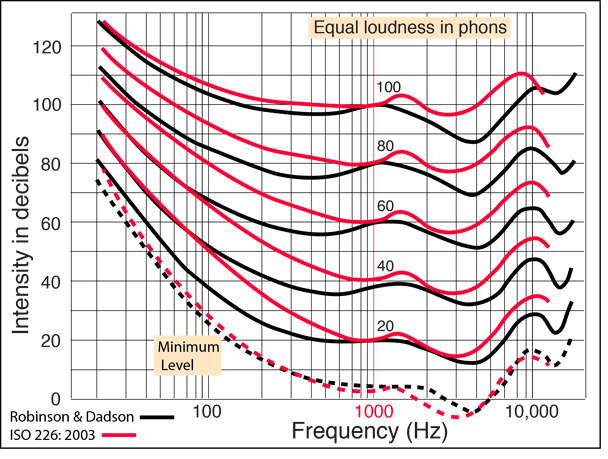
\includegraphics[width=0.8\linewidth]{Chapter_2/figures/equal_loudness_curve.png}
    \caption{Equal-loudness contours comparing the Robinson and Dadson determinations in 1956 (black lines) with the revised ISO~226:2003 standard (red lines). Each contour connects frequency--SPL pairs perceived as equally loud. The label on each contour indicates its loudness level in phons, which corresponds to the SPL of an equally loud 1\,kHz pure tone. The dashed lines represent the minimum threshold of hearing \cite{equal_loudness}.}
  \label{fig:bg_equal_loudness}
\end{figure}

In loudness-related analysis, the \emph{phon} is still not the most convenient end point because it does not provide a linear scale of subjective loudness. A sound of 80 phons is not perceived as twice as loud as one of 40 phons. A more useful perceptual unit is the \emph{sone}, which is designed such that its value is linearly proportional to perceived loudness. A sound of 2 sones is perceived as twice loudness of 1 sones. In practice, there are two common routes to obtain sone values. The first is to convert the loudness level in phons into sones. Table~\ref{tab:dynamics_symbols_phons_sones} gives a few illustrative anchor pairs, while intermediate values are typically obtained by the standard approximation (where the unit of $L_N$ is phons):
\begin{equation}
S =
\begin{cases}
2^{(L_N-40)/10}, & L_N \ge 40,\\[4pt]
(L_N/40)^{2.642}, & L_N < 40.
\end{cases}
\label{eq:bg:phon_to_sone}
\end{equation}
The second route is to approximate perceived loudness directly from physical intensity via Stevens' power law, bypassing the need to read $L_N$ from equal-loudness contours:
\begin{equation}
S = \frac{1}{15.849}\left(\frac{I}{I_0}\right)^{0.3},
\label{eq:bg:stevens_power}
\end{equation}
where $S$ denotes loudness in sones \cite{backus1977acoustical}. In MIR practice, the first route is usually preferable because frequency dependence has already been made explicit through equal-loudness contours and can later be refined further by critical-band modelling.

\subsubsection{Bark-scale and critical bands}

The pure-tone framework above explains how physical level relates to perceived loudness for isolated tones. For musical audio, however, it is not sufficient to treat each FFT bin as an independent loudness event. Singing, piano, and polyphonic textures distribute energy across harmonics, formants, accompaniment, and transients, and the auditory system integrates nearby components within auditory filters whose bandwidth varies with frequency. This is the psychoacoustic motivation for \emph{critical bands} \cite{zwicker1999psychoacoustics}.

The audible frequency range is conventionally organized into 24 critical bands indexed by the Bark scale, a psychoacoustic concept originally proposed by Zwicker in 1961 \cite{zwicker1961subdivision}. Table~\ref{tab:bark_table} shows the approximate relation between Bark index, frequency, and bandwidth. The important point is that Bark is a perceptual frequency coordinate rather than a loudness value: low-frequency bands are relatively narrow in Hz, whereas higher-frequency bands become progressively broader.

\begin{table*}[t]
    \centering
    \caption{Approximate relation between critical-band rate in Bark and frequency in Hz. The full psychoacoustic scale spans 24 critical bands.}
    \label{tab:bark_table}
    \setlength{\tabcolsep}{3pt}
    \fontsize{9pt}{12pt}\selectfont
    \renewcommand{\arraystretch}{1.2}
    \begin{tabular}{ccc|ccc||ccc}
        \hline
        \makecell[c]{\textbf{Critical}\\\textbf{band rate}\\\textbf{$z$ [Bark]}} &
        \makecell[c]{\textbf{Frequency}\\\textbf{$f$ [Hz]}} &
        \makecell[c]{\textbf{$\Delta f$}\\\textbf{[Hz]}} &
        \makecell[c]{\textbf{Critical}\\\textbf{band rate}\\\textbf{$z$ [Bark]}} &
        \makecell[c]{\textbf{Frequency}\\\textbf{$f$ [Hz]}} &
        \makecell[c]{\textbf{$\Delta f$}\\\textbf{[Hz]}} &
        \makecell[c]{\textbf{Critical}\\\textbf{band rate}\\\textbf{$z$ [Bark]}} &
        \makecell[c]{\textbf{Frequency}\\\textbf{$f$ [Hz]}} &
        \makecell[c]{\textbf{$\Delta f$}\\\textbf{[Hz]}} \\
        \hline
        0 & 0    & 100 & 9  & 1080  & 190 & 18 & 4400  & 900  \\
        1 & 100  & 100 & 10 & 1270  & 210 & 19 & 5300  & 1100 \\
        2 & 200  & 100 & 11 & 1480  & 240 & 20 & 6400  & 1300 \\
        3 & 300  & 100 & 12 & 1720  & 280 & 21 & 7700  & 1800 \\
        4 & 400  & 110 & 13 & 2000  & 320 & 22 & 9500  & 2500 \\
        5 & 510  & 120 & 14 & 2320  & 380 & 23 & 12000 & 3500 \\
        6 & 630  & 140 & 15 & 2700  & 450 & 24 & 15500 & --   \\
        7 & 770  & 150 & 16 & 3150  & 550 &    &       &      \\
        8 & 920  & 160 & 17 & 3700  & 700 &    &       &      \\
        \hline
    \end{tabular}
\end{table*}

A common analytic approximation from physical frequency $f$ in kHz to Bark rate $z$ is
\begin{equation}
z(f) = 13\arctan(0.76 f_{\mathrm{kHz}}) + 3.5\arctan\!\left(\frac{f_{\mathrm{kHz}}^2}{7.5^2}\right),
\label{eq:bg:bark_mapping}
\end{equation}
where $f_{\mathrm{kHz}}$ denotes frequency in kHz \cite{pampalk2002content,pampalk2004exploring,zwicker1999psychoacoustics}. This equation defines the Bark coordinate itself. It does not yet compute loudness. 

Once this mapping is available, a linear-frequency spectrogram can be regrouped into Bark bands. If $P(k,t)$ denotes the power at frequency bin $k$ and frame $t$, and $\mathcal{B}_b$ is the set of bins whose center frequencies fall into Bark band $b$, then the Bark spectrogram is
\begin{equation}
P_{\mathrm{Bark}}(b,t) = \sum_{k \in \mathcal{B}_b} P(k,t),
\qquad
\mathcal{B}_b = \{k \mid z_b \le z(f_k) < z_{b+1}\}.
\label{eq:bg:bark_spectrogram}
\end{equation}
This step changes the spectral coordinate system from Hz to critical-band rate. The actual loudness model is introduced in the next subsection, where auditory weighting, spectral spreading, and nonlinear conversion are applied to obtain specific loudness.

\subsubsection{Bark-scale specific loudness and total loudness}
Among psychoacoustic-informed audio representations, Bark-scale specific loudness (BSSL) is designed to represent how perceived loudness is distributed across auditory critical bands, as human perception of loudness is more sensitive to certain frequency bands \cite{zwicker1999psychoacoustics,zwicker2007psychoacoustics}. Because it preserves both spectral location and perceptual magnitude, BSSL is well suited to dynamics-related MIR tasks \cite{narang2024automatic,he2026dynest}.

While several standardized BSSL extraction methods exist, such as DIN 45631/A1:2010 \cite{din45631a1_2010} and ISO 532-1:2017 \cite{iso532_1_2017}, they are primarily optimized for industrial noise assessment and assume stationary sound profiles. In MIR, however, music signals are typically highly polyphonic with negligible background noise. Therefore, the implementation proposed by Pampalk et al. \cite{pampalk2002content, pampalk2004exploring} is widely adopted. The extraction pipeline is defined as follows.

First, the audio is converted to mono, peak-normalised to $-1\,\mathrm{dBFS}$, and resampled to $f_s=22.05\,\mathrm{kHz}$, which preserves sufficient spectral information for MIR tasks. A short-time Fourier transform (STFT) then yields the complex spectrogram $X(k,t)$, where $t$ denotes the frame index and $k$ the frequency-bin index. Then, the power spectrogram $P(k,t)$ is formed using window-energy normalization, and subsequently converted to the decibel scale:
\begin{equation}
P(k,t)=\frac{|X(k,t)|^2}{(\sum_{n=0}^{N-1} w[n])^2},
\end{equation}
\begin{equation}
P_{\mathrm{dB}}(k, t) = \max(0, 10 \log_{10}(P(k, t))).
\end{equation}
To approximate the frequency response of the human outer and middle ear, Terhardt's weighting function $W_{\mathrm{dB}}(f_k)$ \cite{terhardt1979outerear} is applied. This weighting is designed on the power scale (unit is decibel), where $f_k$ denotes the center frequency  (in $\mathrm{kHz}$) of the $k$-th bin:
\begin{equation}
W_{\mathrm{dB}}(f_k) = -3.64\,f_k^{-0.8} + 6.5\,e^{-0.6\,(f_k-3.3)^2} - 10^{-3}\,f_k^{4},
\end{equation}
\begin{equation}
P_W(k,t)=P_{dB}(k,t) \cdot W_{dB}(f_k).
\end{equation}
The weighted power spectrogram $P_W(k,t)$ is then mapped to the Bark scale \cite{zwicker1999psychoacoustics}. Given the $11.05$ kHz Nyquist frequency and the band ranges detailed in Table~\ref{tab:bark_table}, a total of 22 Bark bands are used. Letting the band index be $b \in \{1,\ldots,22\}$, the Bark spectrogram is defined as:
\begin{equation}
B(b,t) = \sum_{k \in \text{Band}b} P_W(k, t).
\end{equation}
Taking account the spectral masking over Bark bands, where a loud sound makes weaker sounds at nearby frequencies harder to preceive, the spreading function $G(\Delta)$ by Schoroeder et al.\cite{schroeder1979masking} is applied:
\begin{equation}
G(\Delta)=15.81 + 7.5(\Delta +0.474) - 17.5\sqrt{1+(\Delta +0.474)^2},
\label{eq:bg:spreading_function}
\end{equation}
\begin{equation}
\widetilde{B}_i(t) = \sum_{i,j=1}^{22} B_i(t) \cdot G(i-j),
\end{equation}
where $\Delta = i-j$ represents the distance between Bark bands. This step reflects a fundamental psychoacoustic principle: loudness perception should not a naive sum of independent narrowband energies, but involves auditory interaction across neighboring critical bands.

Once the Bark-scale excitation is adjusted for the human ears response and spectral spreading, it is converted into a perceptual metric known as \emph{specific loudness}. Following Zwicker's 1999 method \cite{zwicker1999psychoacoustics}, the \emph{specific loudness} is derived by substituting the band-wise Bark excitation $\widetilde{B}(b,t)$ for the pure-tone loudness $L_N$ in Equation~\ref{eq:bg:phon_to_sone}. This yields the BSSL, formally denoted as $N'(b,t)$. Representing the perceived loudness (in sones) for each band $b$ at time $t$, $N'(b,t)$ is defined as:
\begin{equation}
N'(b,t)=
\begin{cases}
2^{(\widetilde{B}(b,t)-40)/10}, & B_{\mathrm{dB}}(b,t)\ge40\\[4pt]
(\widetilde{B}(b,t)/40)^{2.642}, & otherwise.
\end{cases}
\end{equation}
The resulting BSSL, $N'(b,t)$, is a 22-dimensional time-frequency representation of perceived loudness. The corresponding Bark-scale total loudness (BSTL), denoted as $N_{tot}(t)$, collapses the frequency-resolved representation into a single time-varying scalar by integrating over the Bark axis:
\begin{equation}
N_{\mathrm{tot}}(t)=\int_{0}^{22} N'(z,t)\,dz.
\label{eq:bg:total_loudness_cont}
\end{equation}
In other words, BSSL preserves where loudness is located in the auditory spectrum, whereas BSTL retains only the overall perceptual magnitude at each time frame. The two representations are therefore complementary: BSTL is appropriate when a compact loudness curve is sufficient, while BSSL is preferable when the spectral distribution of loudness is expected to carry musically relevant information.

\subsubsection{Other Audio Representations Related to Loudness}
Besides explicit loudness measures, MIR commonly uses spectral representations
that preserve energy information in a more distributed form. The simplest of
these is short-time RMS energy, which summarizes the average signal power
within each analysis frame. RMS is useful as a baseline for tracking local
intensity changes, but it reduces the spectrum to a single value and therefore
cannot reflect how perceived loudness is also influenced by spectral balance,
masking, and timbre. Two vocal passages may have similar RMS energy while
still sounding different in intensity because their energy is distributed
differently across frequency.

For this reason, Mel-based representations are often more informative. A Mel
spectrogram groups spectral energy into perceptually motivated frequency
bands, so each frame retains not only how much energy is present but also
where that energy lies in the spectrum. This is particularly relevant for
singing voice, where changes in vocal effort, resonance, register, or phonation
often affect the spectral envelope as much as the overall level. A log-Mel
spectrogram applies logarithmic compression to these Mel-band energies. This
reduces the dominance of very large amplitudes, makes the representation more
stable across a wide dynamic range, and brings it closer to the nonlinear way
in which intensity is perceived. In practice, linear Mel features preserve
sub-band energy more directly, while log-Mel features are often preferred when
robustness and perceptual relevance are more important.

Compact cepstral features such as MFCCs and BFCCs are derived from log
filterbank energies on the Mel and Bark scales, respectively. They are useful
when a lower-dimensional representation is needed, but the compression also
removes some band-wise detail that may be useful for fine-grained dynamics
analysis. By contrast, the Constant-Q Transform (CQT), which is common in
automatic music transcription, is designed primarily for pitch and harmonic
structure using geometrically spaced frequency bins. It is therefore highly
effective for note-related tasks, but less directly aligned with loudness
analysis, since its design emphasizes pitch resolution rather than perceptual
energy distribution.

\subsection{Dynamics in music score}
\label{sec:bg:dynamics:score}

In Western notation, score dynamics is represented by a small symbolic vocabulary. Static levels include \textit{pp}, \textit{p}, \textit{mf}, and \textit{f}. Gradual transitions include \textit{crescendo} and \textit{diminuendo}. These symbols do not encode fixed decibel values. They encode musical intent. Their realization depends on texture, register, phrasing, repertoire, performer style, and instrument response \cite{kosta2014dynpiano,kosta2016mapping}. This context dependence is precisely why score dynamics remains musically meaningful, but it is also why large-scale annotation and evaluation are difficult.

In this thesis, score dynamics is treated as a beat-synchronous symbolic target. This does not claim that all dynamic markings must occur on beats in music generally. It reflects a practical interface used by the available datasets and by the task formulation of Chapter~5. A beat-synchronous interface makes score dynamics easier to evaluate, easier to align, and easier to write back to a symbolic score.



\begin{table*}[h!]
\centering
\caption[Score-dynamics vocabulary and loudness-related scales]{Illustrative correspondences between score-dynamics vocabulary and loudness-related scales. Phons and sones conversion is referenced from~\cite{backus1977acoustical}.}
\label{tab:dynamics_symbols_phons_sones}
\setlength{\tabcolsep}{4pt}
\fontsize{11pt}{11pt}\selectfont
\renewcommand{\arraystretch}{1.2}
\begin{tabular}{llll}
\toprule
\textbf{Meaning} &
\textbf{Symbols} &
\textbf{Phons} &
\textbf{Sones} \\
\midrule
threshold of pain & \textbf{ffff/sf} & 120 & 128 \\
yelling & \textbf{fff} & 100 & 64 \\
very loud & \textbf{ff} & 90 & 32 \\
loud & \textbf{f} & 80 & 16 \\
normal speaking & \textbf{mf--mp} & 70 & 8 \\
soft & \textbf{p} & 60 & 4 \\
almost a whisper & \textbf{pp} & 50 & 2 \\
whispering & \textbf{ppp} & 40 & 1 \\
threshold of hear & \textbf{pppp/sp} & 0 & 0 \\
\bottomrule
\end{tabular}
\end{table*}


\begin{table*}[h!]
\centering
\scriptsize
\caption[Score-dynamics vocabulary and MIDI velocity scales]{Illustrative correspondences between score-dynamics vocabulary and MIDI velocity scales from representative software documentation, source code, and comparison studies.}
\setlength{\tabcolsep}{2.4pt}
\fontsize{11}{11pt}\selectfont
\renewcommand{\arraystretch}{1.2}
\begin{tabular}{llccccc}
\toprule
Dynamic &
Meaning &
\makecell{Logic Pro\cite{logicpro-stepinput}} &
\makecell{MuseScore\cite{musescore-dynamic-source}} &
\makecell{Sibelius\cite{sibelius7sounds}} &
\makecell{Finale\cite{palamara2020dynamic}} &
\makecell{Dorico\cite{palamara2020dynamic}} \\
\midrule
ffff & threshold of pain    & --  & 127 & --  & 127 & 123 \\
fff  & yelling              & 127 & 126 & 127 & 114 & 119 \\
ff   & very loud            & 112 & 112 & 113 & 101 & 101 \\
f    & loud                 & 96  & 96  & 98  & 88  & 89  \\
mf   & normal speaking      & 80  & 80  & 84  & 75  & 77  \\
mp   & normal speaking      & 64  & 64  & 71  & 62  & 61  \\
p    & soft                 & 48  & 49  & 61  & 49  & 46  \\
pp   & almost a whisper     & 32  & 33  & 39  & 36  & 25  \\
ppp  & whispering           & 16  & 16  & 20  & 23  & 14  \\
pppp & threshold of hear    & --  & 10  & --  & 10  & 5   \\
\bottomrule
\end{tabular}
\label{tab:dyn_midi_main}
\\[0.5ex]
\parbox{0.98\textwidth}{\footnotesize
\textit{Notes.}
(1) Logic Pro current official documentation states that score dynamics are visual only and do not affect playback; the values in the Logic column are Apple's documented \emph{step-input} velocity buttons rather than score-playback dynamics~\cite{logicpro-dynamics-visual,logicpro-stepinput}.
(2) For Finale and Dorico, this table uses the peer-reviewed comparison in~\cite{palamara2020dynamic}; in the official documentation checked for this survey, Finale exposes configurable minimum velocities for dynamic placement, and Dorico exposes playback interpretation options, but I did not locate a vendor-published per-symbol default table.
}
\end{table*}

\begin{table}[h!]
\centering
\scriptsize
\caption[Scalar-based dynamic defaults in LilyPond and music21]{Scalar-based dynamic defaults in LilyPond and music21. LilyPond stores fractions rather than raw MIDI velocities, and the LilyPond integer column is a rounded comparison-only rescaling to 127.}
\setlength{\tabcolsep}{2.4pt}
\fontsize{11}{11pt}\selectfont
\renewcommand{\arraystretch}{1.2}
\begin{tabular}{lcccc}
\toprule
Dynamic &
\makecell{LilyPond\\scalar~\cite{lilypond-midi-doc}}       &
\makecell{LilyPond\\rounded velo~\cite{lilypond-midi-doc}} &
\makecell{music21\\scalar\cite{music21-dynamics-source}}   &
\makecell{music21\\rounded velo~\cite{music21-dynamics-source}} \\
\midrule
sf   & 1.00 & 127 & -- & --    \\
ffff & 0.92 & 117 & 0.95 & 120 \\
fff  & 0.85 & 108 & 0.90 & 114 \\
ff   & 0.80 & 102 & 0.85 & 107 \\
fp   & --   & --  & 0.75 & 95  \\
f    & 0.75 & 95  & 0.70 & 88  \\
mf   & 0.68 & 86  & 0.55 & 69  \\
mp   & 0.61 & 77  & 0.45 & 57  \\
p    & 0.55 & 70  & 0.35 & 44  \\
pp   & 0.49 & 62  & 0.25 & 31  \\
ppp  & 0.42 & 53  & 0.15 & 19  \\
pppp & 0.34 & 43  & 0.10 & 12  \\
\bottomrule
\end{tabular}
\label{tab:dyn_scalar}
\end{table}

\subsection{Dynamics in MIDI}
\label{sec:bg:dynamics:midi}

MIDI velocity is a note-level control parameter attached to note onset. It is often interpreted informally as strike intensity. That is useful, but it should not be conflated with perceived loudness. The mapping from velocity to loudness depends on the instrument mechanism, the sensor calibration, the capture device, and the renderer or recording chain \cite{goebl2003role,dan2006psy,kosta2014dynpiano}. For this reason, the thesis treats MIDI velocity primarily as an \emph{action proxy}. It still remains highly valuable because it is precise, editable, and available on instrumented pianos such as Yamaha Disklavier systems \cite{hawthorne2019maestro}.

This thesis uses MIDI velocity in three ways. In Chapter~3, it is the direct target of symbolic completion. In Chapter~4, it is the target of score-informed refinement from audio. In Chapter~6, it is the target of an exploratory beyond-piano study in which direct labels are scarce and proxy supervision becomes necessary.


\section{Bridging the gap between Dynamics representations}
\label{sec:bg:dynamics:bridge}

\textbf{Why MIDI velocity and score dynamics belong to one thesis:} The two symbolic forms of dynamics solve different problems. MIDI velocity is the natural target for expressive rendering and production workflows. Score dynamics is the natural target for human-readable analysis, notation, and educational feedback. A thesis restricted to only one of them would miss an important part of expressive AMT. By studying both, the dissertation can ask a larger question: how should dynamics be recovered when the available supervision ranges from note-level performance control to weak score-level symbols?

\textbf{Why we cannot directly convert MIDI velocity to Dynamic symbols?}

\subsection{Dynamics depend on musical instruments}
\label{sec:bg:dynamics:piano}

\begin{figure}[h!]
  \centering
  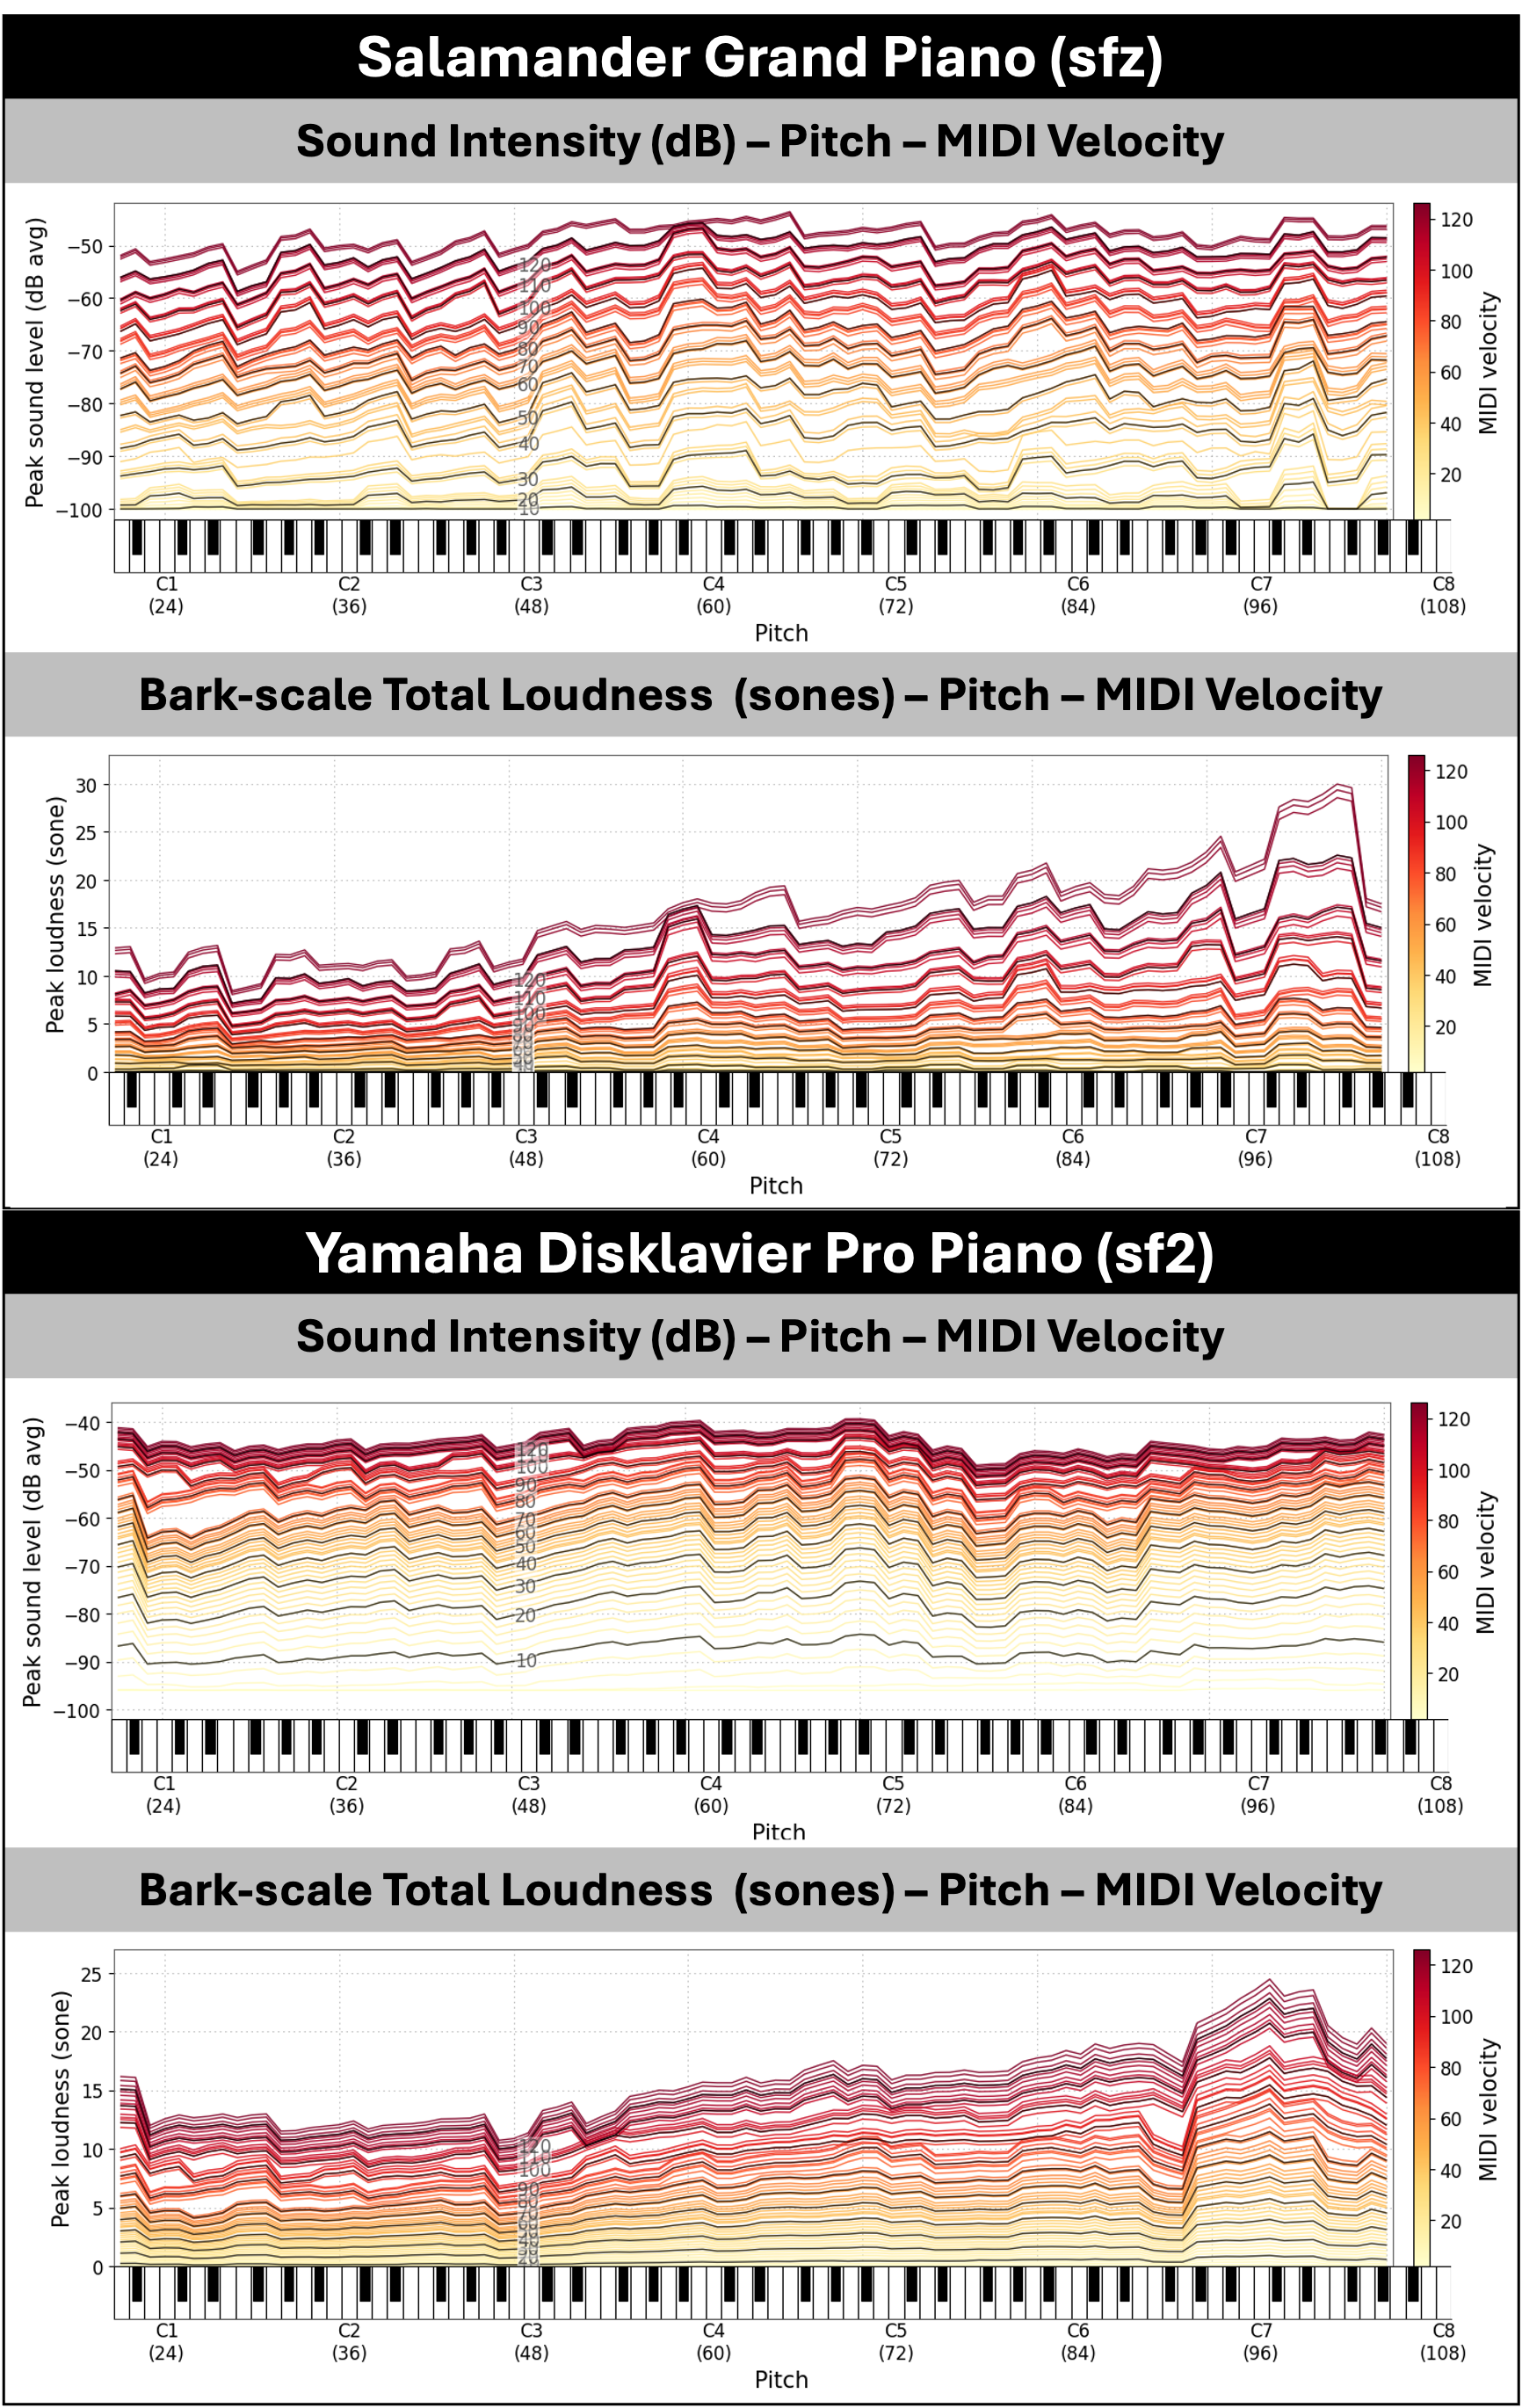
\includegraphics[width=0.99\linewidth]{Chapter_2/figures/soundfont_piano.png}
  \caption{The soundfont analysis of Salamander Grand Piano and Yamaha Disklavier Pro Piano.}
  \label{fig:bg_instruments_sone}
\end{figure}

\begin{figure}[h!]
  \centering
  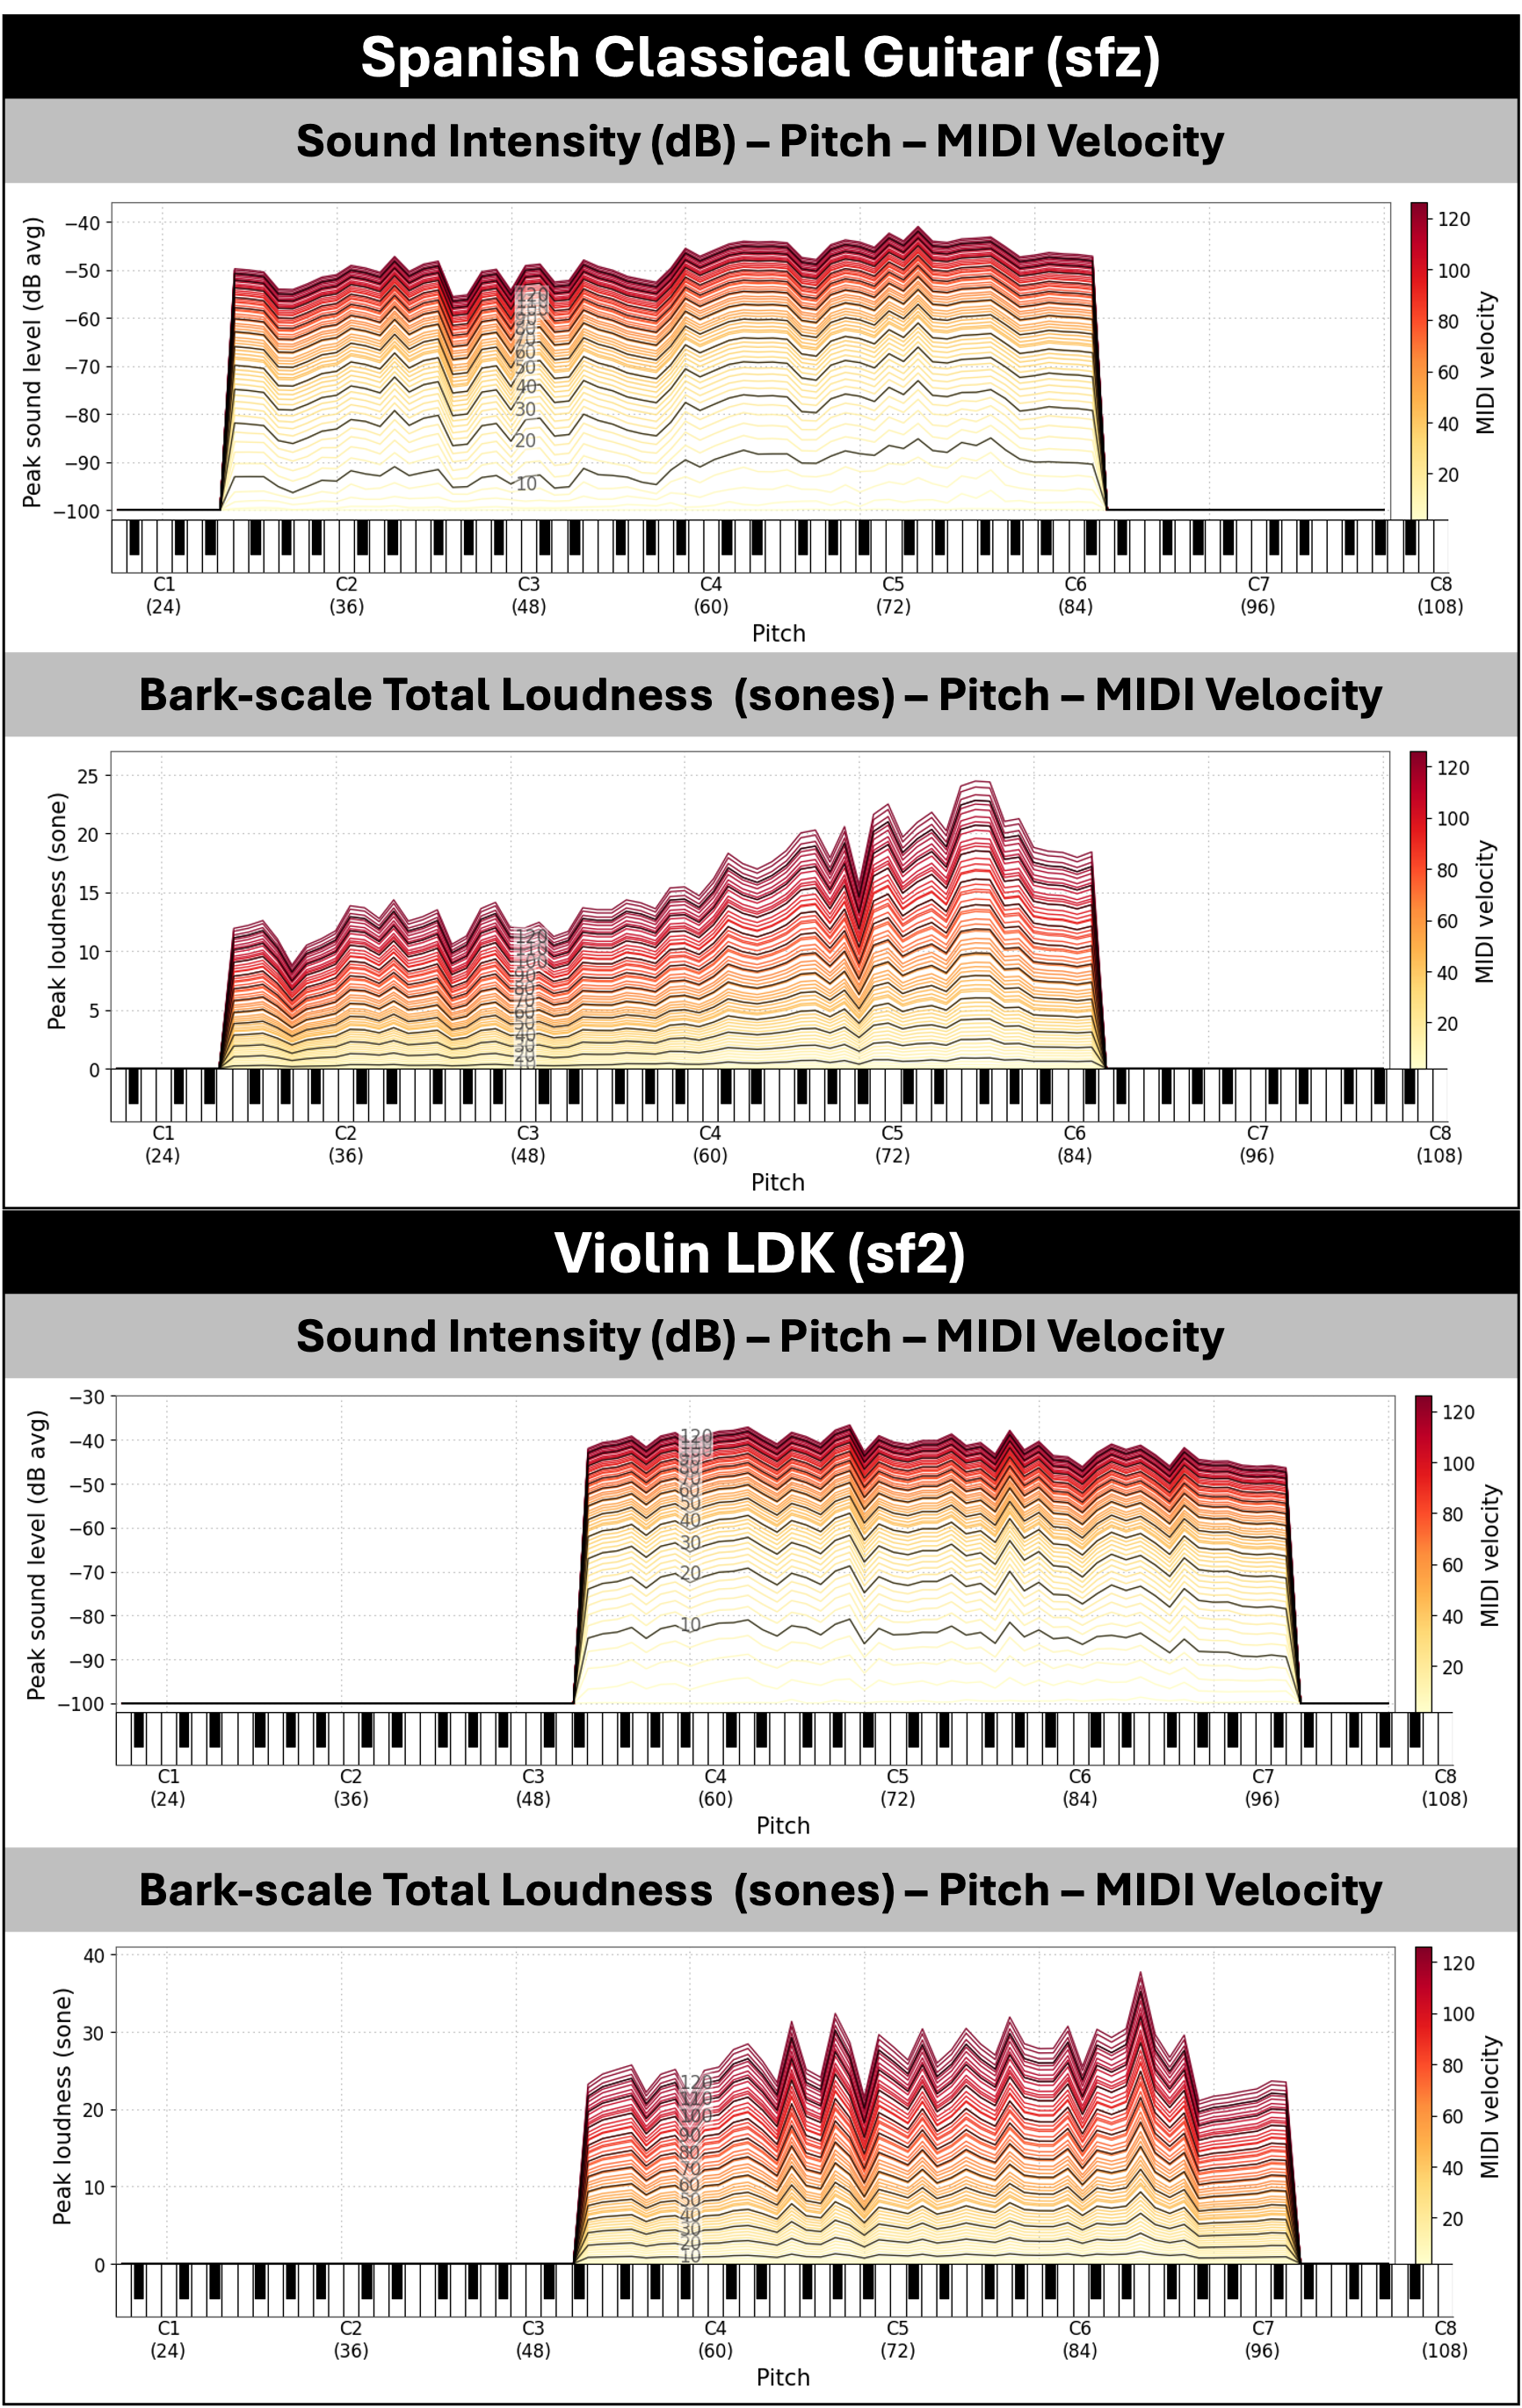
\includegraphics[width=0.99\linewidth]{Chapter_2/figures/soundfont_guitar.png}
  \caption{The soundfont analysis of Spanish Classical Guitar and Violin LDK.}
  \label{fig:bg_instruments_guitar}
\end{figure}

The piano gives this thesis both its main opportunity and its main caution. It is an attractive instrument for dynamics research because note onset is linked to a relatively clear control variable. Piano-performance research often distinguishes between measuring the produced sound and measuring how the sound is produced \cite{goebl2003role}. Within that logic, hammer velocity, MIDI velocity, and resulting loudness are tightly related even though they are not identical. This is one reason why reliable note-level velocity learning is currently concentrated on piano datasets.

At the same time, piano mechanics warn against naive equivalence claims. Even within piano, the relation between MIDI velocity and radiated sound level is non-linear and varies with pitch, touch, instrument, and reproduction chain \cite{goebl2003role}. A note can be louder in the recording because of instrument response, registration, resonance, microphone placement, or rendering conditions rather than because the abstract symbolic velocity is universally \emph{higher}. MIDI velocity is therefore best understood as a useful proxy for performer action at note onset, not as a complete theory of loudness.

\subsection{Human Perceptional Loudness}

The human ear does not hear MIDI velocity or decibels directly. It hears loudness, which depends on frequency content, masking, and temporal integration \cite{zwicker1999psychoacoustics}. This is why the thesis uses perceptually informed front-ends such as Bark-scale specific loudness for audio-based score-dynamics recovery. It is also why the thesis treats score dynamics as a musically underdetermined cue rather than as a fixed physical instruction.

\subsection{Recurring cues and local interpretive events}
\label{sec:bg:dynamics:schemata}

A further distinction from expressive-performance research is valuable here. Some dynamics behaviours are recurrent. They reflect shared schemata such as phrase arches, cadential tapering, local metrical emphasis, or conventional voice balance. Other behaviours are more local and piece-specific. They arise from unusual harmony, texture change, registral surprise, or editorial notation choices. Learning systems can often absorb recurrent cues more readily than these local interpretive events \cite{cancinoChacon2018computational}.

This distinction helps explain why dynamics recovery is inherently uneven across targets. Note-level velocity recovery can track local control values even when their larger symbolic interpretation is unclear. Score-dynamics recovery instead asks for a musically summarized label stream and therefore confronts interpretive ambiguity more directly. This is one reason why the score-facing thread of the thesis requires its own review logic.

\section{Deep Learning and MIR Foundations}
\label{sec:bg:foundations}

\subsection{Recent Progress in AMT and the need for expressive targets}
\label{sec:bg:foundations:performance}

Recent AMT systems are shown as below:

\begin{table*}[t]
\centering

\setlength{\tabcolsep}{2.4pt}
\fontsize{10pt}{11pt}\selectfont
\renewcommand{\arraystretch}{1.2}

\begin{tabular}{
>{\centering\arraybackslash}m{3.0cm}
>{\centering\arraybackslash}m{1.7cm}
>{\centering\arraybackslash}m{2.2cm}
>{\centering\arraybackslash}m{1.2cm}
>{\centering\arraybackslash}m{1.1cm}
>{\centering\arraybackslash}m{1.5cm}
>{\centering\arraybackslash}m{2.0cm}
}
\toprule
Method & Publication & Model & \makecell{F1 \\ frame} & \makecell{F1 \\ note} & \makecell{F1 \\ note\&off} & \makecell{F1 \\ note\&off\&velo} \\
\midrule

\multicolumn{7}{c}{\textbf{MAPS (piano)}} \\
\midrule
OaF \cite{hawthorne2018onsets} & \shortstack{ISMIR \\ 2018} & CRNN & 78.30 & 82.29 & 50.22 & 35.39 \\
Wu et al. \cite{wu2019semantic} & \shortstack{ICASSP \\ 2019} & CNN & 86.73 & -- & -- & -- \\
ADSR \cite{kelz2019adsr} & \shortstack{ICASSP \\ 2019} & CNN + HMM & 77.16 & 81.38 & 56.08 & -- \\
hFT-Trans \cite{toyama2023hft} & \shortstack{ISMIR \\ 2023} & Transformer & 82.89 & 85.14 & 66.34 & 48.20 \\
\midrule

\multicolumn{7}{c}{\textbf{MAESTRO (piano)}} \\
\midrule
OaF$^\dagger$ \cite{hawthorne2018onsets,hawthorne2019maestro} & \shortstack{ISMIR \\ 2018} & CRNN & 87.82 & 94.93 & 79.65 & 76.05 \\
HPT$^\dagger$ \cite{kong2021hpt} & \shortstack{TASLP \\ 2021} & CRNN & 90.15 & 96.77 & 84.45 & 83.02 \\
Semi-CRFs$^\dagger$ \cite{yan2021semicrf} & \shortstack{NeurIPS \\ 2021} & CRNN + Semi-CRF & 91.11 & 96.51 & 88.72 & 87.75 \\
Seq2Seq$^\ddagger$ \cite{hawthorne2021trans,toyama2023hft} & \shortstack{ISMIR \\ 2021} & Transformer & -- & 96.01 & 83.94 & 82.75 \\
HPT-T$^\ddagger$ \cite{kong2021hpt,toyama2023hft} & \shortstack{TASLP \\ 2021} & CRNN & 90.09 & 96.77 & 83.20 & 81.90 \\
HPPNet-sp$^\ddagger$ \cite{wei2022hppnet,toyama2023hft} & \shortstack{ISMIR \\ 2022} & CRNN & 93.15 & 97.18 & 83.80 & 82.24 \\
hFT-Trans$^\ddagger$ \cite{toyama2023hft} & \shortstack{ISMIR \\ 2023} & Transformer & 93.24 & 97.44 & 90.53 & 89.48 \\
Transkun v2$^\ddagger$ \cite{yan2024semicrf} & \shortstack{ISMIR \\ 2024} & Transformer + Semi-CRF & 95.35 & 98.32 & 93.48 & 92.94 \\
\midrule

\multicolumn{7}{c}{\textbf{MusicNet (multi-instrument)}} \\
\midrule
Wu et al. \cite{wu2019semantic} & \shortstack{ICASSP \\ 2019} & CNN & 73.70 & -- & -- & -- \\
ReconVAT \cite{cheuk2021reconvat,gardner2022mt3} & \shortstack{ACM MM \\ 2021} & U-Net & 48.0 & 29.0 & 11.0 & -- \\
MT3 \cite{gardner2022mt3} & \shortstack{ICLR \\ 2022} & Transformer & 68.0 & 50.0 & 33.0 & -- \\
PerceiverTF$^\S$ \cite{lu2023perceivertf} & \shortstack{ICASSP \\ 2023} & Perceiver + Transformer & 63.7 & 46.1 & 29.0 & -- \\
PF2N$^\S$ \cite{kim2025pf2n} & \shortstack{Mathematics \\ 2025} & Perceiver + PF2N & 64.5 & 47.5 & 30.7 & -- \\
\bottomrule
\end{tabular}

\vspace{0.5ex}
\parbox{0.98\linewidth}{\footnotesize
$^\dagger$ Historical MAESTRO results reported on the earlier MAESTRO split/re-evaluation used by HPT and Semi-CRF papers. \\
$^\ddagger$ Results reported directly on MAESTRO v3.0.0 or re-tabulated on MAESTRO v3.0.0 by later papers. \\
$^\S$ PF2N evaluates multi-instrument settings with an additional requirement that the predicted instrument label match the ground truth. These rows are therefore not directly comparable to the original instrument-agnostic MT3 MusicNet scores.
}
\caption{Representative AMT results across MAPS, MAESTRO, and MusicNet, showing that velocity-aware transcription remains substantially harder than note transcription.}
\label{tab:amt_sota}
\end{table*}


\subsection{Performance research as a precursor to expressive MIR}
\label{sec:bg:foundations:precursor}

Expressive MIR inherits many of its core questions from music performance research. Long before deep-learning AMT, performance studies had already shown that phrase structure, meter, local accent, and instrumental constraints shape both timing and dynamics \cite{goebl2003role,cancinoChacon2018computational}. This older literature matters because it clarifies that expressive labels are not decorative metadata attached to a note list. They are traces of interpretation. As a result, expressive AMT must confront questions of target definition, representational choice, and evaluation legitimacy that are already familiar in performance science.


\subsection{From note transcription to expressive transcription}
\label{sec:bg:foundations:evolution}

Classical AMT focused on pitch estimation and note boundary detection. Deep-learning AMT expanded this to high-resolution piano transcription, event-based transcription, and increasingly robust note modelling across datasets \cite{amt2019ov,hawthorne2018onsets,hawthorne2021trans,kong2021hpt,toyama2023hft,yan2021semicrf,yan2024semicrf}. This evolution matters for the present thesis because dynamics recovery does not start from zero. It builds on a field that can already recover a large part of the note structure reliably, especially for piano. The remaining gap is that expressive targets are still much less mature than note targets.

Seen from this perspective, expressive AMT is not a separate field detached from AMT. It is the next layer of symbolic recovery once note content and timing become reasonably stable. The thesis therefore positions its contributions as extensions of AMT toward expressive and editable symbolic outputs rather than as alternatives to note transcription.

\subsection{Common neural architectures in MIR}
\label{sec:bg:foundations:architectures}

Several neural architecture families recur across MIR and across this thesis. Convolutional neural networks are effective for local time--frequency pattern extraction. They remain a strong default when the task depends on local spectral cues or sparse spatial structure. Transformer models use self-attention to model longer-range dependencies and have become increasingly important for AMT and beat tracking \cite{vas2017attn,hawthorne2021trans,toyama2023hft,foscarin2024beat}. Conformer-style models combine self-attention with convolution and are attractive when both local detail and wider context matter \cite{gulati2020conformer}.

For this thesis, the main issue is not textbook taxonomy. It is \emph{inductive bias}. Sparse symbolic matrices invite U-Net-like locality. Event-level correction invites token-based representations and attention over note events. Phrase-level score dynamics invites perceptual front-ends and long temporal context. The architecture choices made later are therefore motivated by the structure of the target rather than by model fashion.

\subsection{Multi-task learning, negative transfer, and mixture-of-experts}
\label{sec:bg:foundations:mtl}

Multi-task learning is attractive when several outputs share information. In MIR, it can reduce duplicate computation and encourage a common representation. However, it can also cause negative transfer when tasks prefer different acoustic cues or different temporal context. This risk is especially important for Chapter~5, where dynamic estimation and beat tracking must coexist in one model. Mixture-of-experts methods address this by combining shared representation learning with task-specific routing \cite{ma2018mmoe}. The MMoE decoder used later in Chapter~5 follows precisely this logic.

\subsection{Multi-scale modelling and long-context design}
\label{sec:bg:foundations:multiscale}

Many music tasks are inherently multi-scale. Note onset detection needs fine temporal resolution. Phrase-level dynamics needs longer context. Beat and downbeat tracking lie somewhere in between. A single temporal scale is rarely optimal for all of them. Multi-scale architectures address this by providing parallel or hierarchical pathways with different effective receptive fields \cite{li2023frame}. In the present thesis, this principle appears most directly in Chapter~5, but the broader idea also motivates segment-length design choices in Chapter~3 and the residual late-correction principle in Chapter~4.

\section{Representations and Alignment Across Audio, MIDI, and Score}
\label{sec:bg:repr}

% \begin{figure}[t]
%   \centering
%   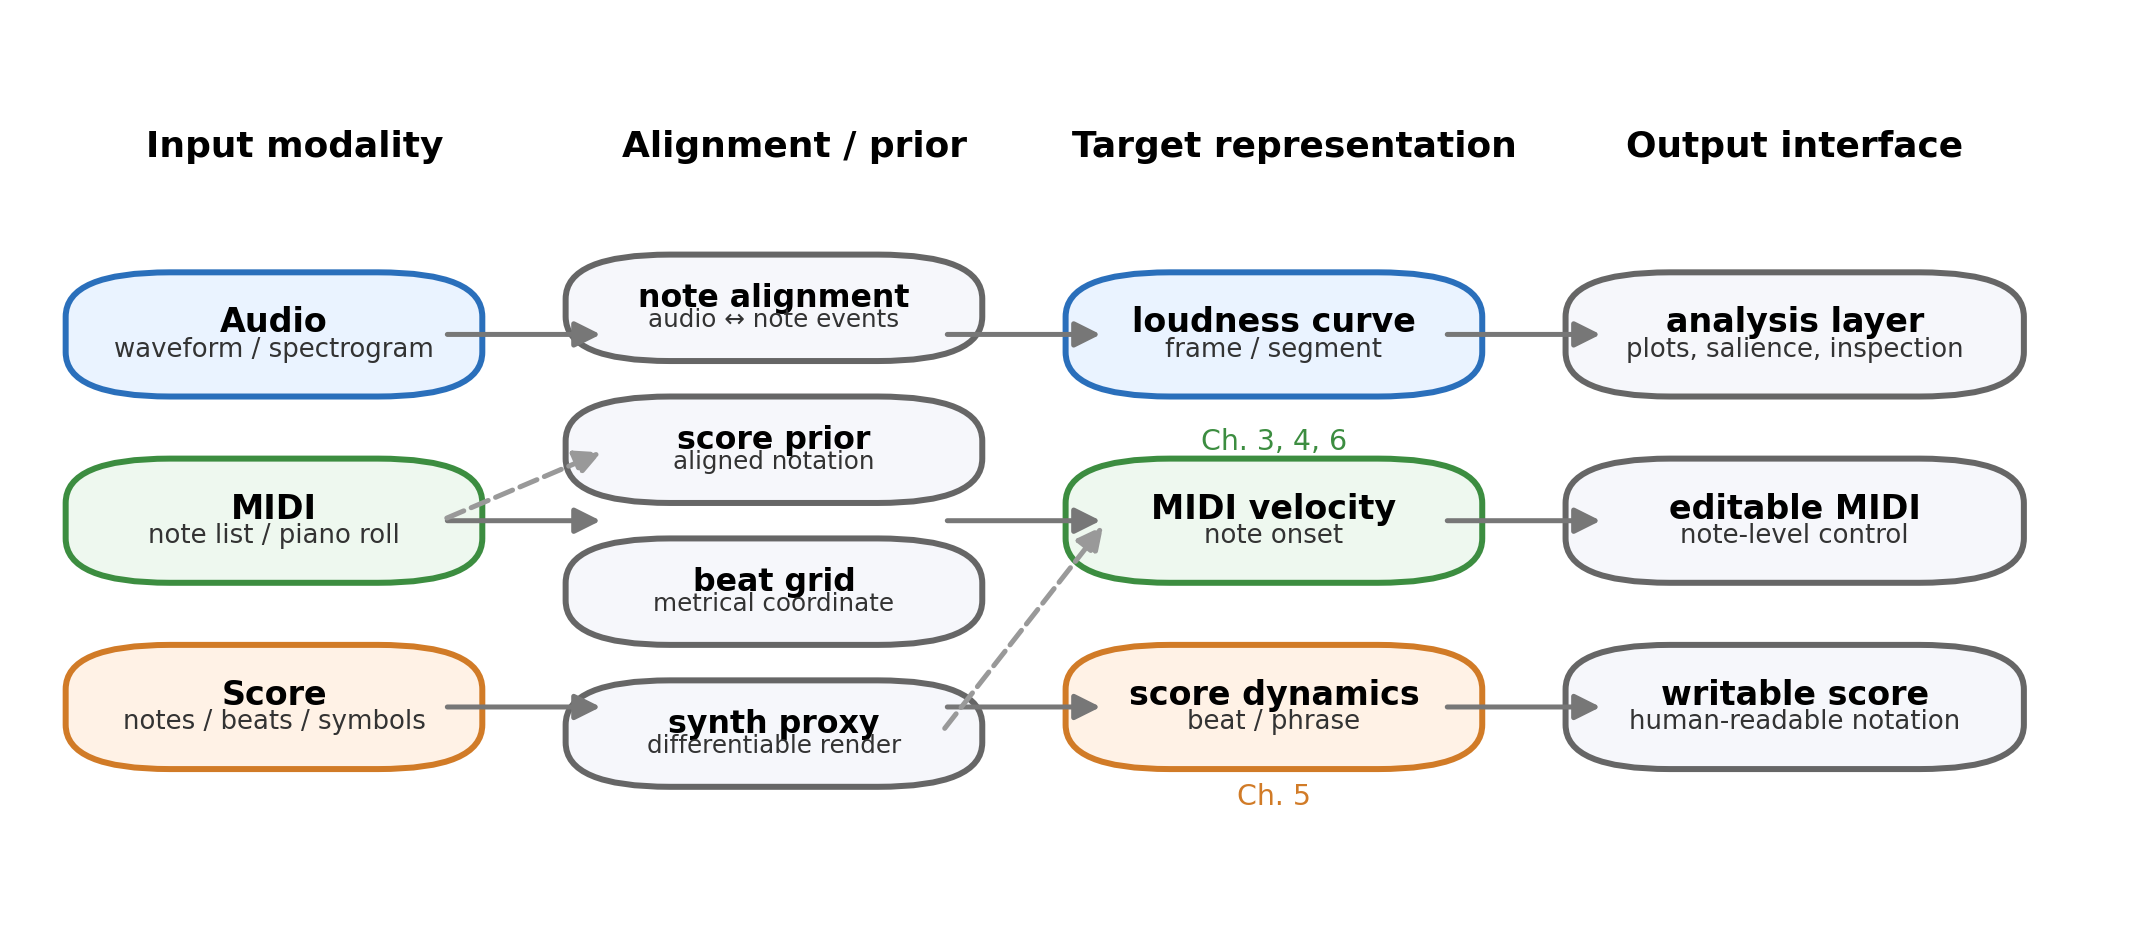
\includegraphics[width=0.99\linewidth]{Chapter_2/figures/representation_chain.png}
%   \caption{Shared representation logic of the thesis. Different chapters start from different inputs, use different forms of structural support, and target different dynamics representations. The figure makes the transition from modality to output interface explicit.}
%   \label{fig:bg_representation_chain}
% \end{figure}

\subsection{Audio representations}
\label{sec:bg:repr:audio}

Most transcription systems operate on time--frequency representations. Common choices include magnitude spectrograms, log-Mel spectrograms, and variants of constant-Q or perceptual front-ends \cite{amt2019ov}. Log-Mel remains a strong general-purpose choice because it supports both pitch-related and onset-related modelling. However, it is not necessarily the best inductive bias for loudness-oriented tasks. For dynamics estimation, perceptually grounded features may reduce the gap between physical signal variation and perceived intensity. This motivates the comparison between log-Mel and Bark-scale specific loudness in Chapter~5.

\subsection{Symbolic and score representations}
\label{sec:bg:repr:symbolic}

The thesis uses two main symbolic interfaces. For note-level tasks, MIDI is often rasterized into piano-roll-like matrices indexed by pitch and time. Onset rolls, frame rolls, and velocity rolls provide a convenient representation for sparse note events and are especially suitable for 2D models \cite{he2025filling}. For score-informed tasks, symbolic note information can also be represented as tokens carrying time, pitch, note state, and optionally score-derived attributes \cite{kim2023score}. These tokenized representations become more natural when the model acts on note events rather than on dense frame grids.

For score-level tasks, the score provides a different representational interface. Beats and downbeats form a musically meaningful coordinate system. Dynamic symbols can then be attached to this coordinate system as sparse, interpretable labels. Chapter~5 adopts exactly this beat-synchronous interface.

\subsection{Temporal units}
\label{sec:bg:repr:units}

The same acoustic event can be indexed in several ways. That choice is not neutral. It determines what is being predicted and how the prediction should be evaluated.

\begin{figure}[t]
  \centering
  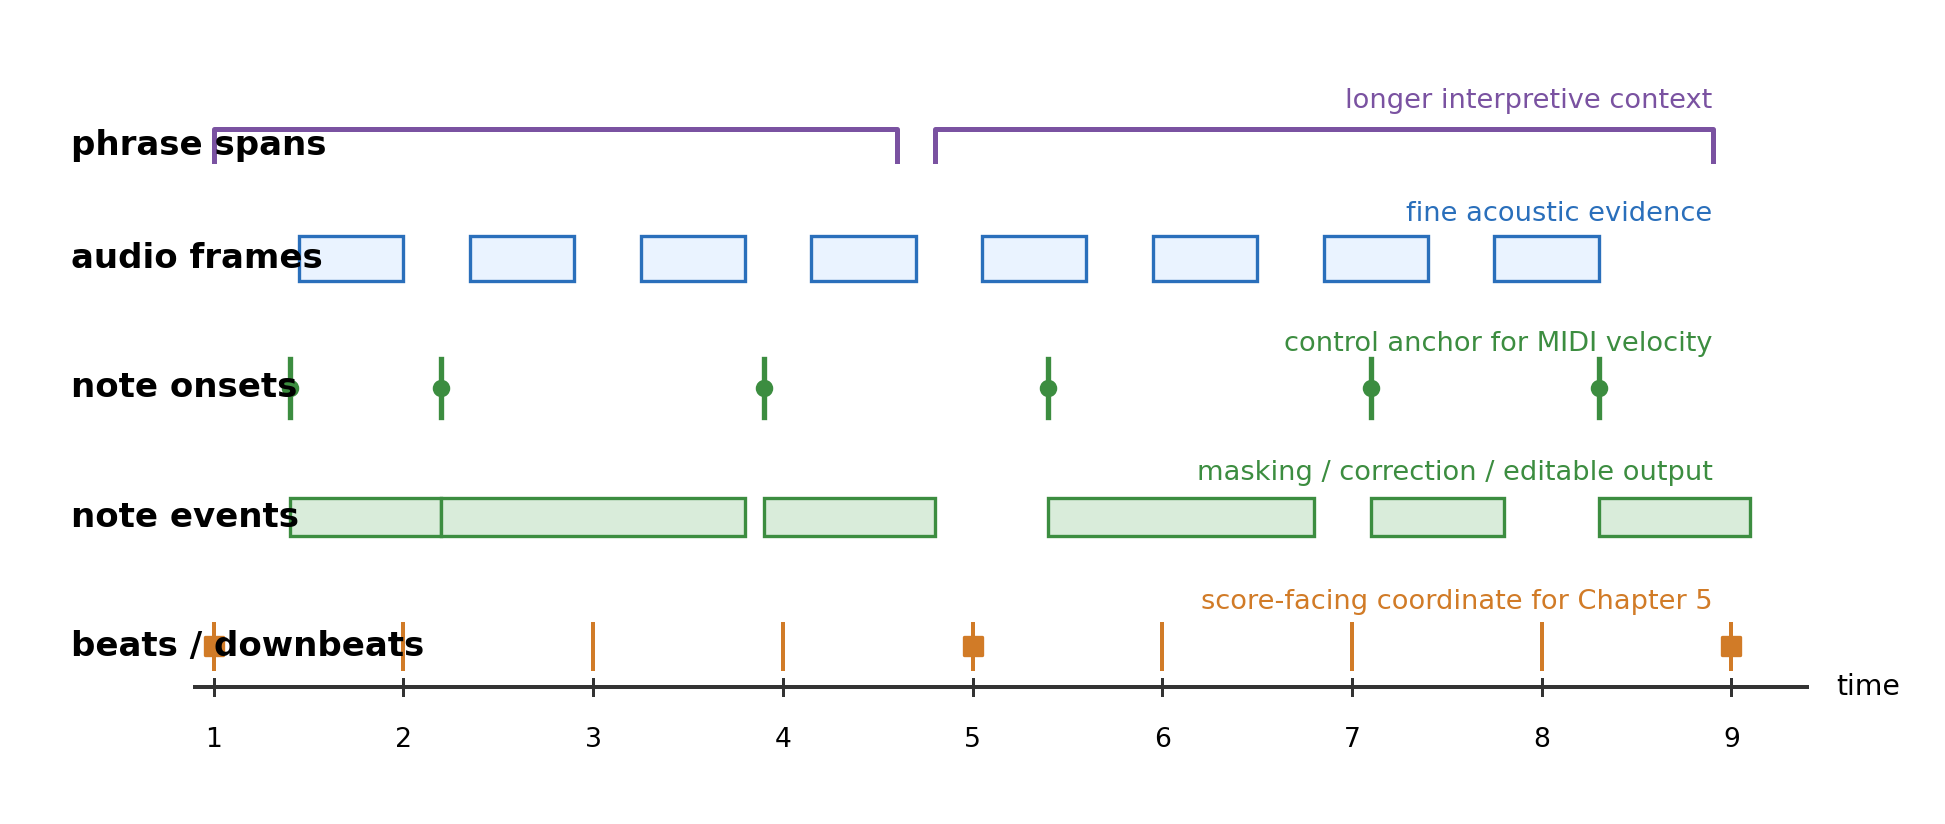
\includegraphics[width=0.98\linewidth]{Chapter_2/figures/temporal_units.png}
  \caption{Temporal units that recur across the thesis. Audio frames support fine acoustic evidence. Note onsets and note events support control-level modelling. Beats and downbeats provide score-facing coordinates. Phrase spans capture longer interpretive context.}
  \label{fig:bg_temporal_units}
\end{figure}

\begin{table}[t]
\centering
\caption{Temporal units that recur across the thesis.}
\label{tab:bg_temporal_units}
\small
\setlength{\tabcolsep}{4pt}
\renewcommand{\arraystretch}{1.15}
\begin{tabularx}{\textwidth}{l l X}
\toprule
\textbf{Unit} & \textbf{Where it appears} & \textbf{Why it matters} \\
\midrule
Frame & audio loudness and acoustic features & Captures fine temporal evidence but is too dense for many score-facing targets \\
Note onset & MIDI velocity and AMT outputs & Natural coordinate for action-level intensity control \\
Note event & symbolic completion and correction & Supports note-wise masking, correction, and editable symbolic output \\
Beat & score dynamics and metrical tracking & Main coordinate for human-readable dynamic labels \\
Downbeat & score dynamics and phrase context & Anchors bar-level organization and change-point interpretation \\
Phrase / segment & expressive interpretation & Explains longer contextual shaping that cannot be reduced to isolated notes \\
\bottomrule
\end{tabularx}
\end{table}

\subsection{Alignment, priors, and validity}
\label{sec:bg:repr:alignment}

Alignment is not a minor preprocessing detail. It determines what the supervision actually means and whether evaluation is legitimate. For note-level velocity estimation, note onsets and offsets must be aligned with either the audio or the reference score. Instrumented piano datasets provide this directly through synchronized audio--MIDI capture \cite{hawthorne2019maestro}. In score-informed settings, the aligned score supplies the note events that should receive velocity values. This makes note-level masked evaluation possible.

For score dynamics, the critical coordinate is the beat grid. Beat-level alignment may come from a reference score, from manual annotations, or from the model itself. This alignment is essential because score dynamics is rarely meaningful as an unconstrained frame-wise label stream. It becomes interpretable once mapped to beats, bars, and phrase-level change points.

The thesis also uses the notion of a \emph{prior} in a broader sense. In Chapter~4, the prior is an aligned score that stabilizes note-level correction. In Chapter~5, the prior is the metrical coordinate system that makes score-facing labels meaningful. In Chapter~6, the prior takes a different form: differentiable MIDI-to-audio synthesis provides an indirect route from predicted control values back to the observed signal. These are different mechanisms, but they all serve the same purpose. They inject structure into an otherwise underdetermined dynamics problem.

\section{Thread A: Note-Level MIDI Velocity Recovery}
\label{sec:bg:threadA}

\subsection{Expressive rendering and humanisation}
\label{sec:bg:threadA:rendering}

Expressive performance rendering aims to generate expressive control signals from symbolic input. Many systems predict timing, dynamics, and sometimes articulation jointly \cite{jeong2019virtuosonet,borovik2023scoreperformer}. These models are important because they show that expressive performance can be learned from symbolic structure. At the same time, they reveal a practical limitation for the present thesis. Joint expressive rendering may alter more than the user wants. In production or corpus-upgrading settings, the desired operation is often narrower: preserve the notes and timing, and recover only the missing dynamics layer. This narrower, controllable objective is the entry point for Chapter~3.

\subsection{Symbolic velocity completion and prediction}
\label{sec:bg:threadA:symbolic}

Symbolic velocity completion assumes that the note sequence is already known and that the missing variable is note-level velocity. Early work used rule-based or statistical approaches \cite{berndt2010modelling}. More recent work formulates the task with deep learning, including convolutional autoencoders and sequence-to-sequence models with attention \cite{kuo2021velocity,kim2023piano}. Diffusion-based note-intensity estimation has also been explored in related score-informed settings \cite{kim2023diffvel}.

A central challenge is the sparsity of symbolic piano-roll data. Dense frame grids contain large silent regions. A model that treats all cells equally can waste much of its capacity. This is one reason why the image-like formulation of Chapter~3 is attractive. It allows sparse note structure to be processed with U-Net-style locality while still supporting wider context.

\subsection{Audio-driven velocity estimation within AMT}
\label{sec:bg:threadA:amt}

Velocity recovery from audio has become increasingly feasible for piano because large aligned datasets exist with sensor-recorded note velocities \cite{hawthorne2019maestro}. Representative velocity-enabled AMT systems include OaF, HPT, hFT-Trans, and event-based models \cite{hawthorne2018onsets,hawthorne2021trans,kong2021hpt,toyama2023hft,yan2021semicrf,yan2024semicrf}. Related work also studies robustness, semi-supervised learning, and parameter-efficient piano transcription \cite{maman2022general,edwards2024general,strahl2024semi,wei2022hppnet,wang2025multitask}.

Despite strong progress, note-level velocity remains more fragile than note pitch and onset estimation. Domain shift in piano timbre, microphone placement, room acoustics, and recording chain degrades the mapping from acoustic evidence to velocity more severely than the mapping from acoustic evidence to pitch. This fragility is one of the main motivations for the score-informed correction strategy of Chapter~4.

\subsection{Score-informed MIDI velocity estimation and correction}
\label{sec:bg:threadA:scoreinf}

Score-informed velocity estimation assumes that an aligned score is available together with performance audio. Historically, this line of work developed partly because early AMT systems focused on notes and offered limited support for reliable velocity estimation \cite{amt2013ov}. Early systems used hand-designed measurements or parametric estimation strategies \cite{dan2006psy,goebl2003role,szeto2005finding,ewert2011est}. Later work introduced restricted Boltzmann machines, score-informed non-negative matrix factorization, diffusion-based note-level estimation, and FiLM-conditioned deep models \cite{van2014pred,jeong2017note,jeong2018timbre,kim2023diffvel,kim2023score,kim2024method,simonetta2022acoustics}.

A key pattern in this literature is \emph{feature fusion}. Score information is injected into the acoustic model during feature extraction. This can improve accuracy, but it also ties the score-informed method tightly to a particular backbone. The present thesis instead emphasizes \emph{late correction}. A correction module can attach to an existing AMT system and refine its velocity estimate while leaving the backbone largely unchanged. This is the design stance developed in Chapter~4.

\subsection{Piano bias and the beyond-piano problem}
\label{sec:bg:threadA:beyond}

Reliable velocity supervision is still strongly piano-centric. Instrumented pianos make note-level velocity available at scale, but comparable datasets for other instruments are scarce. This creates both a training bias and an evaluation bias. Transfer beyond piano must therefore confront two bottlenecks: missing labels and instrument-dependent mappings between performer action, timbre, and loudness.

The important point is that beyond-piano failure is not only ordinary domain shift. It is a measurement problem. Outside piano, even defining what a ``ground-truth'' note-level control signal should be can be difficult. This distinction is essential for the honest positioning of Chapter~6.

\subsection{Cross-instrument velocity estimation with proxy supervision}
\label{sec:bg:threadA:proxy}

When true note-level velocity labels are unavailable, one route is to supervise the predicted control indirectly through audio reconstruction. Differentiable MIDI-to-audio synthesis, including DDSP-style systems, makes this increasingly plausible because a model can be penalized after its predicted velocities are rendered back to sound \cite{engel2020ddsp}. The appeal is clear. It turns a missing-label problem into a proxy-supervision problem.

The danger is equally clear. A proxy objective can reward compatibility with the synthesizer more than compatibility with real instrumental control. Reconstruction error is therefore not the same thing as accurate velocity recovery. Chapter~6 adopts this route explicitly as an exploratory study. Its value lies in opening the beyond-piano question honestly, not in claiming that proxy supervision has already replaced true labels.

\section{Thread B: Beat-Synchronous Score-Dynamics Recovery}
\label{sec:bg:threadB}

\subsection{From performed loudness to score dynamics}
\label{sec:bg:threadB:loudness}

Computational modelling of dynamics has a long history in expressive performance research \cite{cancinoChacon2018computational}. Rather than focusing only on note-level control, this line of work studies how performed loudness relates to symbolic dynamic markings and phrase structure. Kosta and collaborators showed both the usefulness and the ambiguity of this relationship \cite{kosta2014dynpiano,kosta2016mapping,kosta2018mazurkabl}. Other work has further analysed dynamic principles in piano performance \cite{jones2023probingdyn}.

From a machine-learning perspective, score-dynamics recovery can be framed as classification or structured sequence labelling. The input is audio. The output is a sequence of dynamic symbols or dynamic regimes. In the MazurkaBL line of work, the performed-loudness side of this mapping is typically extracted through sone-based psychoacoustic processing rather than raw amplitude, precisely because the target concerns perceived intensity rather than unweighted energy \cite{kosta2017thesis}. The challenge is that these labels are sparse, relative, and musically contextual rather than physically absolute. This is one reason why a beat-synchronous formulation is more natural than direct frame-wise regression of continuous loudness.

\subsection{Change points and dynamic segmentation}
\label{sec:bg:threadB:changepoints}

Dynamic markings rarely behave as independent frame labels. They form local regimes that persist over spans of music, and musical meaning often lies in the transitions between those regimes. Change-point detection therefore plays an important role. It supports segmentation, interpretation, and the recovery of phrase-level dynamic structure \cite{kosta2018mazurkabl,kosta2017thesis}. In Chapter~5, change points are estimated jointly with dynamic levels so that a score-facing output includes both local states and their transitions.

\subsection{Beat and downbeat tracking as structural coordinates}
\label{sec:bg:threadB:metrical}

Beat and downbeat tracking has a mature literature. Earlier systems often relied on convolutional features followed by probabilistic post-processing such as dynamic Bayesian networks \cite{bock2020deconstruct,zhao2022beat}. More recent systems use stronger deep encoders and can reduce reliance on heavy post-processing \cite{foscarin2024beat}. For this thesis, beat and downbeat tracking is not only a useful auxiliary task. It is the coordinate system that makes score dynamics interpretable, comparable, and writable back to a score.

\subsection{Joint estimation and multi-task learning}
\label{sec:bg:threadB:joint}

Dynamics estimation and metrical estimation are closely related but not identical. Dynamic labels are easier to interpret on a beat grid, yet beat tracking itself needs precise temporal localization that differs from the longer context required for phrase-level dynamics. This mismatch creates an ideal test case for multi-scale and multi-task design. Shared encoders can capture common information, but negative transfer must be controlled. Mixture-of-experts style decoders are therefore well motivated for this thread \cite{ma2018mmoe}. Chapter~5 adopts exactly this view by combining a multi-scale encoder with task-aware routing.

\section{Common Architecture for AMT and Related Tasks}
\label{sec:bg:common_arch}

The later chapters use different architectures, but they draw from a relatively small set of reusable design ideas.

\subsection{Sparse 2D modelling with U-Net and attention}
\label{sec:bg:common_arch:unet}

When symbolic music is rasterized as piano-roll matrices, the resulting representation is sparse but still has local spatial structure. U-Net-style architectures are well suited to this combination because they preserve fine local detail through skip connections while aggregating larger context through the encoder--decoder path. Windowed attention can then be added to improve feature aggregation without the full cost of global attention \cite{shen2023linear,chen2022hts}. This toolbox underlies Chapter~3.

\subsection{Token-based correction modules}
\label{sec:bg:common_arch:tokens}

When note events are already known, a dense frame representation is not always the most efficient interface. A note-token representation can focus modelling capacity on the events that actually require correction. This principle is especially suitable for late correction, where the aim is to adjust a preliminary estimate rather than to solve transcription end to end. It underlies the score-informed Transformer module of Chapter~4.

\subsection{Perceptual front-ends and long-context audio modelling}
\label{sec:bg:common_arch:perceptual}

For score-dynamics recovery, the relevant signal is closer to perceived loudness than to raw pitch content alone. Perceptual front-ends such as Bark-scale specific loudness preserve not only a scalar loudness trajectory but also the Bark-wise distribution of loudness across the spectrum. They can therefore provide a better inductive bias and can also reduce model size by compressing the frequency dimension. This compactness is not only an implementation detail. It enables substantially longer audio segments, which are crucial for phrase-level context in Chapter~5.

\subsection{MMoE and task-aware routing}
\label{sec:bg:common_arch:mmoe}

Shared representations are useful across related tasks, but they are not sufficient when tasks prefer different temporal or acoustic cues. MMoE provides a practical compromise between full parameter sharing and fully separate models \cite{ma2018mmoe}. It lets tasks draw differently from a shared expert pool. This principle is central to the multi-task audio-only model of Chapter~5 and is conceptually aligned with the thesis-level idea of modular expressive label recovery.

\subsection{Differentiable synthesis and proxy losses}
\label{sec:bg:common_arch:proxy}

Proxy supervision becomes relevant when the target control parameter is musically meaningful but rarely labeled. Differentiable synthesis provides one route. A network predicts control values, those values are rendered back to audio through a differentiable synthesizer, and losses are applied in the signal domain. In a DDSP-style setting, this can provide regression pressure even when direct control annotations are absent \cite{engel2020ddsp}.

For expressive AMT, this strategy is attractive but delicate. It makes missing-label learning possible, yet it also ties the learning signal to the adequacy of the synthesizer. The thesis therefore treats proxy losses as a method family with explicit limits, not as a universal substitute for true note-level control labels.

\section{Datasets, Evaluation, and Reproducibility Constraints}
\label{sec:bg:dataeval}

\begin{table}[h]
\centering
\caption{Representative datasets relevant to expressive label recovery in this thesis.}
\label{tab:dataset_comparison}

\setlength{\tabcolsep}{2.4pt}
\fontsize{11pt}{11pt}\selectfont
\renewcommand{\arraystretch}{1.2}

\begin{tabularx}{\textwidth}{
l l
c c c
c c c c
}
\toprule
\multirow{2}{*}{\textbf{Dataset}} &
\multirow{2}{*}{\textbf{Instr.}} &
\multicolumn{3}{c}{\textbf{Statistic}} &
\multicolumn{4}{c}{\textbf{Modality}} \\
\cmidrule(lr){3-5} \cmidrule(lr){6-9}
&
& \textbf{Hours}
& \makecell{\textbf{Perfor-}\\\textbf{mance}}
& \makecell{\textbf{Compos-}\\\textbf{itions}}
& \textbf{MIDI}
& \makecell{\textbf{Velo.}}
& \textbf{Score}
& \makecell{\textbf{Dyn.}} \\
\midrule

\addlinespace[2pt]
ATEPP \cite{zhang2022atepp}
& piano
& 1007
& 11742
& 1580
& \cmark
& \cmark
& \cmark\ 43\%
& \warn\ 43\% \\
\addlinespace[4pt]
\multicolumn{9}{>{\raggedright\arraybackslash}p{\dimexpr\textwidth-2\tabcolsep\relax}}
{\hspace{1em}\warn\ Audio is from YouTube URLs (avail. vary); score dynamics are not explicitly verified.} \\
\addlinespace[2pt]
\midrule

\addlinespace[2pt]
ASAP \cite{foscarin2020asap}
& piano
& 92
& 1068
& 222
& \cmark
& \cmark
& \cmark
& \warn \\
\addlinespace[4pt]
\multicolumn{9}{>{\raggedright\arraybackslash}p{\dimexpr\textwidth-2\tabcolsep\relax}}
{\hspace{1em}\warn\ Score dynamics (and other expressive markings) are not verified.} \\
\addlinespace[2pt]
\midrule

\addlinespace[2pt]
MAESTRO v3 \cite{hawthorne2019maestro}
& piano
& 172
& 1276
& 864
& \cmark
& \cmark
& \xmark
& \xmark \\
\addlinespace[4pt]
\multicolumn{9}{>{\raggedright\arraybackslash}p{\dimexpr\textwidth-2\tabcolsep\relax}}
{\hspace{1em}\cmark\ High-quality piano dataset, recorded on Yamaha Disklavier pianos.} \\
\addlinespace[2pt]
\midrule

\addlinespace[2pt]
SMD v2 \cite{smd}
& piano
& 4.7
& 50
& 50
& \cmark
& \cmark
& \xmark
& \xmark \\
\addlinespace[4pt]
\multicolumn{9}{>{\raggedright\arraybackslash}p{\dimexpr\textwidth-2\tabcolsep\relax}}
{\hspace{1em}\cmark\ Often used for cross-dataset evaluation; recorded on Yamaha Disklavier pianos.} \\
\addlinespace[2pt]
\midrule

\addlinespace[2pt]
MAPS \cite{maps}
& piano$^\dagger$ 
& 17.9
& 270
& 208
& \cmark
& \cmark
& \xmark
& \xmark \\
\addlinespace[4pt]
\multicolumn{9}{>{\raggedright\arraybackslash}p{\dimexpr\textwidth-2\tabcolsep\relax}}
{\hspace{1em} $^\dagger$ Statistics are computed only on the ENSTDkAm and ENSTDkCl subsets (solo piano), recorded on Yamaha Disklavier pianos.} \\
\addlinespace[2pt]
\midrule

\addlinespace[2pt]
MazurkaBL \cite{kosta2018mazurkabl}
& piano
& 110
& 2000
& 44
& \xmark
& \xmark
& \cmark
& \cmark \\
\addlinespace[4pt]
\multicolumn{9}{>{\raggedright\arraybackslash}p{\dimexpr\textwidth-2\tabcolsep\relax}}
{\hspace{1em}\cmark\ Dynamics and Expressive labels are explicitly verified. All Chopin compositions.}\\
\addlinespace[2pt]
\midrule

\addlinespace[2pt]
Vienna4x22 \cite{goebl1999vienna4x22}
& piano
& 2.3
& 88
& 4
& \cmark
& \cmark
& \cmark
& \cmark \\
\addlinespace[4pt]
\multicolumn{9}{>{\raggedright\arraybackslash}p{\dimexpr\textwidth-2\tabcolsep\relax}}
{\hspace{1em}\cmark Contains 4 compositions from Chopin, Schubert and Mozart, each 22 performances.} \\
\addlinespace[2pt]
\midrule

\addlinespace[2pt]
Batik-plays-Moz.~\cite{hu2023batik}
& piano
& 3.7
& 36
& 36
& \cmark
& \cmark
& \cmark
& \cmark \\
\addlinespace[4pt]
\multicolumn{9}{>{\raggedright\arraybackslash}p{\dimexpr\textwidth-2\tabcolsep\relax}}
{\hspace{1em}\cmark Contains 12 Mozart sonatas represented as 36 movement-level score--performance pairs. The public repository provides MIDI, MusicXML scores, and match files; corresponding audio recordings are commercially available rather than distributed in the repository. The current GitHub README reports a total duration of 223.28\,min (3.72\,h).} \\
\addlinespace[2pt]
\midrule

\addlinespace[2pt]
MSMD \cite{dorfer2018msmd}
& piano
& 15
& 479
& 479
& \cmark
& \xmark
& \cmark
& \xmark \\
\addlinespace[4pt]
\multicolumn{9}{>{\raggedright\arraybackslash}p{\dimexpr\textwidth-2\tabcolsep\relax}}
{\hspace{1em}\warn\ Synthesized audio; MIDI is derived from digital scores rather than human performance.} \\
\addlinespace[2pt]
\midrule

\addlinespace[2pt]
GuitarSet \cite{xi2018guitarset}
& guitar
& 3.0
& 360
& 30
& \cmark
& \xmark
& \xmark
& \xmark \\
\addlinespace[4pt]
\multicolumn{9}{>{\raggedright\arraybackslash}p{\dimexpr\textwidth-2\tabcolsep\relax}}
{\hspace{1em}\cmark\ Good quality electric guitar dataset.} \\
\addlinespace[2pt]
\midrule

\addlinespace[2pt]
GOAT \cite{loth2025goat}
& guitar
& 5.9
& 172
& n/a.
& \cmark
& \xmark
& \cmark
& \xmark \\
\addlinespace[4pt]
\multicolumn{9}{>{\raggedright\arraybackslash}p{\dimexpr\textwidth-2\tabcolsep\relax}}
{\hspace{1em}\cmark\ Usage may still be constrained by copyright or redistribution terms.} \\
\addlinespace[2pt]
\midrule

\addlinespace[2pt]
\makecell[l]{Fran\c{c}ois\\Leduc} \cite{francoisleduc_zenodo}
& guitar
& 4.0
& 78
& n/a.
& \cmark
& \xmark
& \warn
& \xmark \\
\addlinespace[4pt]
\multicolumn{9}{>{\raggedright\arraybackslash}p{\dimexpr\textwidth-2\tabcolsep\relax}}
{\hspace{1em}\warn\ By request only; released files include audio--MIDI pairs, but not the original scores.} \\
\addlinespace[2pt]
\midrule

\addlinespace[2pt]
GAPS \cite{riley2024gaps}
& guitar
& 14.1
& 300
& 300
& \cmark
& \xmark
& \cmark
& \xmark \\
\addlinespace[4pt]
\multicolumn{9}{>{\raggedright\arraybackslash}p{\dimexpr\textwidth-2\tabcolsep\relax}}
{\hspace{1em}\warn\ Audio is collected from YouTube URLs (availability may vary).} \\
\addlinespace[2pt]
\midrule

\addlinespace[2pt]
MusicNet \cite{thickstun2017musicnet}
& ensemble
& 34.1
& 330
& 121
& \cmark
& \warn
& \xmark
& \xmark \\
\addlinespace[4pt]
\multicolumn{9}{>{\raggedright\arraybackslash}p{\dimexpr\textwidth-2\tabcolsep\relax}}
{\hspace{1em}\cmark\ Classical multi-instrument recordings; note labels are aligned from score via DTW; reference MIDI is available; \warn\ alignment noise exists; velocity is score-derived and not performance control.} \\
\addlinespace[2pt]
\midrule

\addlinespace[2pt]
MID-FiLD \cite{ryu2024midfild}
& ensemble
& n/a.
& 4477
& 4477
& \cmark
& \cmark
& \xmark
& \xmark \\
\addlinespace[4pt]
\multicolumn{9}{>{\raggedright\arraybackslash}p{\dimexpr\textwidth-2\tabcolsep\relax}}
{\hspace{1em}\warn\ Synthesized audio; MIDI is derived from digital scores rather than human performance.} \\
\addlinespace[2pt]

\bottomrule
\end{tabularx}
\end{table}

\subsection{Dataset modalities and what each chapter can learn}
\label{sec:bg:dataeval:modalities}

The thesis relies on datasets with very different modality combinations. Audio--MIDI datasets such as MAESTRO support supervised note-level velocity learning. Cross-dataset piano corpora such as SMD and MAPS stress generalization under changed recording conditions. Score-aligned corpora such as MazurkaBL support score-facing dynamics research because they provide beat-level structure and expressive annotations. Other datasets are valuable but incomplete for the present thesis because they may lack reliable note-level velocity, verified score dynamics, or stable redistribution conditions.

These modality differences are not an implementation detail. They determine which claim can be made at all. Chapter~3 needs reliable symbolic velocity targets. Chapter~4 additionally needs an aligned score. Chapter~5 needs score-facing dynamics with metrical structure. Chapter~6 needs candidate non-piano corpora, but cannot assume direct velocity supervision of MAESTRO quality.

\subsection{Evaluation for MIDI velocity}
\label{sec:bg:dataeval:velocity}

Velocity should be evaluated at note level rather than by naive frame-wise error. Otherwise, long sustained notes dominate the metric. Standard statistics include mean absolute error and related dispersion measures \cite{kuo2021velocity,kim2024method}. However, numerical accuracy alone is not sufficient. A model can achieve a decent average error while producing over-smoothed or mechanically centered dynamics. Distribution-sensitive measures, visual inspection, and listening tests therefore play an important complementary role. This is especially evident in Chapter~3, where perceptual differences are not always fully captured by raw error.

Cross-dataset evaluation is also essential. Piano type, velocity calibration, microphone placement, and room acoustics all affect the mapping from performance action to recorded signal. A model that performs well only on the training dataset does not yet solve expressive AMT in a practical sense.

\subsection{Evaluation for score dynamics}
\label{sec:bg:dataeval:scoredyn}

Score dynamics is usually evaluated as classification on a musically meaningful grid. F1 score is common because the class distribution is imbalanced and because some symbols occur much less frequently than others \cite{kosta2017thesis}. In the present thesis, beat-synchronous evaluation is especially important because it avoids arbitrary frame-level tolerance choices and aligns the prediction target with how the annotations are actually used in music notation.

Evaluation remains inherently limited by label ambiguity. Different editors or annotators may disagree on dynamic markings. Different editions of the same piece may contain different expressive symbols. This does not invalidate the task, but it does mean that score-dynamics performance must be interpreted with awareness of the annotation convention behind the dataset.

\subsection{Evaluation under proxy supervision}
\label{sec:bg:dataeval:proxy}

When direct note-level velocity labels are absent, evaluation becomes weaker and must be stated more carefully. Audio reconstruction error after differentiable synthesis is informative, but it is not equivalent to accurate velocity recovery. A proxy-supervised study should therefore separate three questions. Does the synthesized audio become more plausible? Do the predicted control values display musically reasonable distributions and relative trends? Does any anchor subset with stronger labels show positive transfer?

This evaluation logic is directly relevant to Chapter~6. The contribution of that chapter is exploratory because the supervision and evaluation are weaker than in the piano chapters. Making that weakness explicit strengthens the thesis. It does not weaken it.

\subsection{Reproducibility, alignment quality, and licensing}
\label{sec:bg:dataeval:repro}

Expressive AMT research is strongly constrained by data quality and licensing. Many scores are copyrighted. Many recordings cannot be redistributed freely. Some datasets rely on external URLs or derived alignments whose long-term availability is uncertain. Alignment quality is another major factor. A method may fail not because the dynamics model is poor, but because the score or beat alignment is noisy.

For this reason, reproducible expressive AMT research should document preprocessing, alignment assumptions, train/validation/test protocols, and all modality constraints clearly. The later thesis chapters follow this principle, and the final conclusion of the dissertation treats these constraints as design considerations rather than afterthoughts.

\section{Summary of Gaps and Thesis Requirements}
\label{sec:bg:summary}

The literature reviewed above motivates six thesis requirements.

\begin{itemize}
    \item \textbf{R1 Preserve note content and timing while recovering dynamics.} Many expressive systems modify several performance dimensions jointly. The present thesis instead treats dynamics as a refinement or annotation layer. This requirement is most visible in Chapters~3, 4, and 6.

    \item \textbf{R2 Support heterogeneous data-availability settings.} Real corpora differ widely in what is available: symbolic MIDI only, audio plus aligned score, audio only, or audio with only proxy supervision. This requirement motivates the overall design of Chapters~3--6.

    \item \textbf{R3 Respect representation differences explicitly.} Loudness, MIDI velocity, and score dynamics are linked but not identical. The target representation must therefore be chosen deliberately and defended in each chapter. This requirement spans the whole thesis.

    \item \textbf{R4 Use musically meaningful coordinates for score-level outputs.} Score dynamics should not be treated as an arbitrary frame-wise label stream. It should be expressed on a beat-synchronous interface that supports interpretation, evaluation, and symbolic writing. This requirement motivates Chapter~5.

    \item \textbf{R5 Evaluate with both numerical and musical evidence.} Objective metrics are necessary but not always sufficient. Listening tests, qualitative inspection, distributional behaviour, and cross-dataset evaluation remain important. This requirement is visible in Chapters~3, 5, and 6.

    \item \textbf{R6 Treat beyond-piano transfer as a supervision problem rather than ordinary domain shift.} Once true note-level velocity labels disappear, proxy supervision may be necessary, but its claims must remain limitation-aware. This requirement motivates the explicit exploratory framing of Chapter~6.
\end{itemize}

Together, these requirements define the dissertation stance. The next chapters respond to them under deliberately different assumptions rather than as stages of one pipeline. Chapter~3 studies symbolic-only note-level recovery. Chapter~4 studies score-informed note-level refinement from audio. Chapter~5 studies audio-only recovery of beat-synchronous score dynamics. Chapter~6 probes beyond-piano note-level recovery when direct labels are no longer available.

	\include{Chapter_3/Chap3}
	\include{Chapter_4/Chap4}
	\include{Chapter_5/Chap5}
	\include{Chapter_6/Chap6}
	\chapter{Conclusion}
\label{ch:conclusion}

This chapter concludes the thesis by summarizing findings, limitations, and future research directions.

\section{Summary of Contributions}
TODO.

\section{Limitations}
TODO.

\section{Future Work}
TODO.


\cleardoublepage
\renewcommand{\bibname}{Reference}
\bibliographystyle{IEEEbib}
\bibliography{reference}
\end{document}
